\documentclass[11pt,a4paper]{article}

\usepackage{gastex}
\usepackage{etoolbox}
% \newcommand{\showLoesung}{2} %<---als Schalter
%\newcommand{\showInhalt}{1} %<---als Schalter

\usepackage{alltt,moreverb,amsmath,enumerate}
\usepackage[normalem]{ulem}
\usepackage[T1]{fontenc}
\usepackage{ae,aecompl} %helvet,mathptm
%\usepackage[left=15mm,right=15mm,top=20mm,bottom=20mm]{geometry}
\usepackage[margin=.5in]{geometry}
%\usepackage[latin1]{inputenc} % f�r Linux
\usepackage[utf8]{inputenc} % Umlaute etc. direkt schreiben (unter Windows)
\usepackage[german]{babel}
\usepackage[url]{oth-logoPNG}
%\usepackage{i2sym,i2ams}

\usepackage{tikz}
\usetikzlibrary{arrows,shapes,trees,positioning,automata,decorations.pathreplacing,decorations.pathmorphing}
\usepackage{tkz-graph}
\usepackage{color}

\usepackage{longtable}
\usepackage{tabularx}

%\usepackage{epic}
%\usepackage{eepic}
\usepackage{comment,ifthen}
\usepackage{../include/todo}

\usepackage[T1]{fontenc}
\usepackage{textcomp}

\usepackage{listings}                   % Listings in Core-Erlang und Maude
\usepackage{lstmisc}

\usepackage{epic}                       % Bildbefehle (picture)
%\usepackage{eepic}                      % erweiterte Bildbefehle

\usepackage{bbm}                        % Mengensymbole (N,C,R,B)
\usepackage{latexsym}                   % zusaetzliche Mathesymbole
\usepackage{amsmath}                    % Mathepaket von der AMS
\usepackage{amstext}
\usepackage{amsfonts}
\usepackage{stmaryrd}                   % zusaetzliche Mathesymbole
\usepackage{mathtools}
\usepackage{amsthm}
\usepackage{cancel}

\usepackage{hyperref}
\usepackage{url}                        % Zum Setzen von URLs in typewriter-face

\pagestyle{empty}

\let\epsilon=\varepsilon
\let\phi=\varphi

\frenchspacing

\setlength{\parindent}{0pt}
\setlength{\textwidth}{18.6cm}
\setlength{\textheight}{26.5cm}
\setlength{\hfuzz}{1mm}

%%% Read dates of assignments from file
\usepackage{xparse}
\ExplSyntaxOn
\ior_new:N \g_hringriin_file_stream

\NewDocumentCommand{\ReadFile}{mm}
 {
  \hringriin_read_file:nn { #1 } { #2 }
  \cs_new:Npn #1 ##1
   {
    \str_if_eq:nnTF { ##1 } { * }
      { \seq_count:c { g_hringriin_file_ \cs_to_str:N #1 _seq } }
      { \seq_item:cn { g_hringriin_file_ \cs_to_str:N #1 _seq } { ##1 } }
   }
 }

\cs_new_protected:Nn \hringriin_read_file:nn
 {
  \ior_open:Nn \g_hringriin_file_stream { #2 }
  \seq_gclear_new:c { g_hringriin_file_ \cs_to_str:N #1 _seq }
  \ior_map_inline:Nn \g_hringriin_file_stream
   {
    \seq_gput_right:cx 
     { g_hringriin_file_ \cs_to_str:N #1 _seq }
     { \tl_trim_spaces:n { ##1 } }
   }
  \ior_close:N \g_hringriin_file_stream
 }

\ExplSyntaxOff

\ReadFile{\uebungsabgabe}{../skel/UEBUNGSABGABE.def}

%%% Read subject info from file
\newcommand{\dozent}[1]{\def\DOZENT{#1}}
\newcommand{\tutoren}[1]{\def\TUTOREN{#1}}
\newcommand{\vorlesung}[1]{\def\VORLESUNG{#1}}
\newcommand{\semester}[1]{\def\SEMESTER{#1}}

\InputIfFileExists{../skel/VORLESUNG.def}{\providecommand{\TUTOREN}{}}%
{\typeout{***********}
 \typeout{Warnung: Kein File vorhanden, das die Vorlesung spezifiziert!}
 \typeout{Spezifikation muss daher im Text des Blattes oder ueber die
          Tastatur erfolgen.}
 \typeout{***********}}

\def\Uebung#1#2#3{
  \othLehrstuhlLogo[\DOZENT]
  \begin{center}
	{~\\[-2em]\Large\bf \VORLESUNG}\\[0.5em]
    \LARGE --~Tutorium #1 (Übung #2)~--\\[4mm]
  \
  \normalsize
  \textbf{#3}
    \rule{\textwidth}{0.1pt}\\[1cm]
  \end{center}
}

\def\Hinweis#1{
	{~\\[-3em]\bf Hinweis: }
	\begin{minipage}[t]{16.5cm}
	#1
	\end{minipage}\\[1em]
    \rule{\textwidth}{0.1pt}
}

\def\Tipps#1{
	{~\\[-3em]\bf Tipps: }
	\begin{minipage}[t]{16.5cm}
	#1
	\end{minipage}\\[1em]
    \rule{\textwidth}{0.1pt}
}
  
\def\MyHeader{
  \othLehrstuhlLogo[Prof.~Dr.~rer.~nat.~Carsten~Kern]%[Carsten~Kern,~Stefan~Rieger]
}

\newcommand{\sem}[1]{[\![#1\,]\!]}

\def\aufgabe#1#2{\subsection*{Aufgabe #1 (#2)}\par}
\def\endaufgabe{}

\newenvironment{loesung}{\subsection*{L\"osungsvorschlag:}}{}
\newenvironment{hinweis}{}{}
\ifthenelse{\isundefined{\showLoesung}}{\excludecomment{loesung}}{\pagestyle{plain}\excludecomment{hinweis}}

\newenvironment{tipps}{}{}
\ifthenelse{\isundefined{\showTipps}}{\excludecomment{tipps}}{\excludecomment{hinweis}}

\newenvironment{inhalt}{\subsection*{Kommentar:}}{}
\ifthenelse{\isundefined{\showInhalt}}{\excludecomment{inhalt}}{}

\long\def\Exercise#1#2{\begin{exercise}{#1}#2\end{exercise}}

\def\underbar#1{%
  \setbox0=\hbox{#1}%
  \dimen0=\dp0\relax%
  \dp0=0pt%
  \setbox0=\hbox{\underline{\box0}}%
  \dp0=\dimen0\relax%
  \box0%
  }

\makeatletter
\def\@makeunderbar[#1]#2{\expandafter\def\csname#1\endcsname{\underbar{#2}}}
\def\makeunderbar{\@ifnextchar[{\@makeunderbar}{\@makeunderbar[]}}
\makeatother

\def\T{\mathrm{T}}
\def\P{\mathrm{P}}
\def\CT{\mathrm{CT}}
\def\COp{\mathrm{COp}}

\makeunderbar{Comp}
\makeunderbar{Ops}
\makeunderbar{trans}
\makeunderbar[strans]{s-trans}
\makeunderbar[ntrans]{n-trans}
\makeunderbar{fix}

\def\labelenumi{\alph{enumi})}
\let\<=\langle
\let\>=\rangle

\parindent=0pt
\parskip=1ex

\definecolor{javared}{rgb}{0.6,0,0} % for strings
\definecolor{javagreen}{rgb}{0.25,0.5,0.35} % comments
\definecolor{javapurple}{rgb}{0.5,0,0.35} % keywords
\definecolor{javadocblue}{rgb}{0.25,0.35,0.75} % javadoc
 
\lstset{language=C++,
basicstyle=\ttfamily\footnotesize,
keywordstyle=\color{javapurple}\bf,
stringstyle=\color{javared},
commentstyle=\color{javagreen}\it\bf,
morecomment=[s][\color{javadocblue}]{/**}{*/},
numbers=left,
numberstyle=\tiny\color{gray},
stepnumber=1,
numbersep=10pt,
tabsize=3,
showspaces=false,
showstringspaces=false}

\usepackage{enumitem}
\usepackage{algpseudocode}
\usepackage{caption}
\usepackage{subcaption}
\usepackage{placeins}

\begin{document}
\thispagestyle{empty}

\Uebung{4}{5}{Simon Thelen}{04. November 2021}  % FIXME: Blattnummer, Datum, Zeit

%%%%%%%%%%%%%%%%%%%%%%%%%%%%%%%%%%%%%%%%%%%%%%%%%%%%%%%%%%%%%%%%%%%%%%

\ifcsdef{showLoesung}{
\textbf{Bitte beachten Sie:} Die Lösungen können trotz sorgfältiger Prüfung Fehler enthalten.
Bei Fragen oder Unklarheiten kontaktieren Sie bitte den Tutor oder Dozenten in Tutorien, Übungen oder nach Vorlesungen.
}{}


\begin{aufgabe}{1}{Heap-Operationen}
    \begin{enumerate}[label=\alph*)]
        \item \label{it:ex} Gegeben sei folgendes Array: $(32, 4, 12, 71, 32, 66, 19, 15)$. Führen Sie händisch \textsc{BuildMaxHeap} auf diesem Array aus.
        Geben Sie den resultierenden Heap an.
        \item Entfernen Sie von Hand aus dem resultierenden Heap aus Teilaufgabe a) mittels \textsc{Heapify} die drei größten Elemente.
        \item Mit Heapify lassen sich Werte in den Heap hineinsickern, um die Heap-Eigenschaft wiederherzustellen.
        Gegeben sei die folgende Funktion, die einen Wert solange im Heap aufsteigen lässt, bis die Heap-Eigenschaft wiederhergestellt ist.
        \begin{lstlisting}[language=c++]
void bubbleUp(int a[], int i) {
    while (i > 0 && a[(i - 1) / 2] < a[i]) {
        swap(a[i], a[(i - 1) / 2]);
    }
}
        \end{lstlisting}
        Erweitern Sie unter Zuhilfenahme der obigen Funktion die Heap-Datenstruktur um weitere Operationen:
        \begin{itemize}
            \item \textsc{Remove}: Entfernt den Wert, der sich an einem gegebenen Array-Index befindet, aus dem Heap.
            \item \textsc{Insert}: Fügt einen einzelnen Wert in einen bestehenden Heap ein (Sie können davon ausgehen, dass das zugrundeliegende Array Platz für das neue Element hat).
        \end{itemize}
        Überlegen Sie sich, wie diese Operationen mit Worst-Case-Laufzeit $O\big(\log(n)\big)$ umgesetzt werden können.
        Die Heap-Eigenschaft soll nach jedem Aufruf einer der Operationen weiterhin an allen Stellen des Heaps gelten.
        Implementieren Sie die Operationen in Pseudocode oder einer Programmiersprache Ihrer Wahl.
        \item Gegeben sei der resultierende Heap aus Teilaufgabe a).
        Führen Sie von Hand die folgenden Operationen hintereinander aus: \textsc{Remove(2)}, \textsc{Insert(66)}.
        Wie sieht der Heap nach den einzelnen Operationen jeweils aus?
    \end{enumerate}
\end{aufgabe}

\ifcsdef{showLoesung}{\newpage}{}

\begin{loesung}
    \begin{enumerate}
        \item \ \\
        \begin{figure}[h!]
            \centering
            \begin{subfigure}[b]{0.23\textwidth}
                \centering
                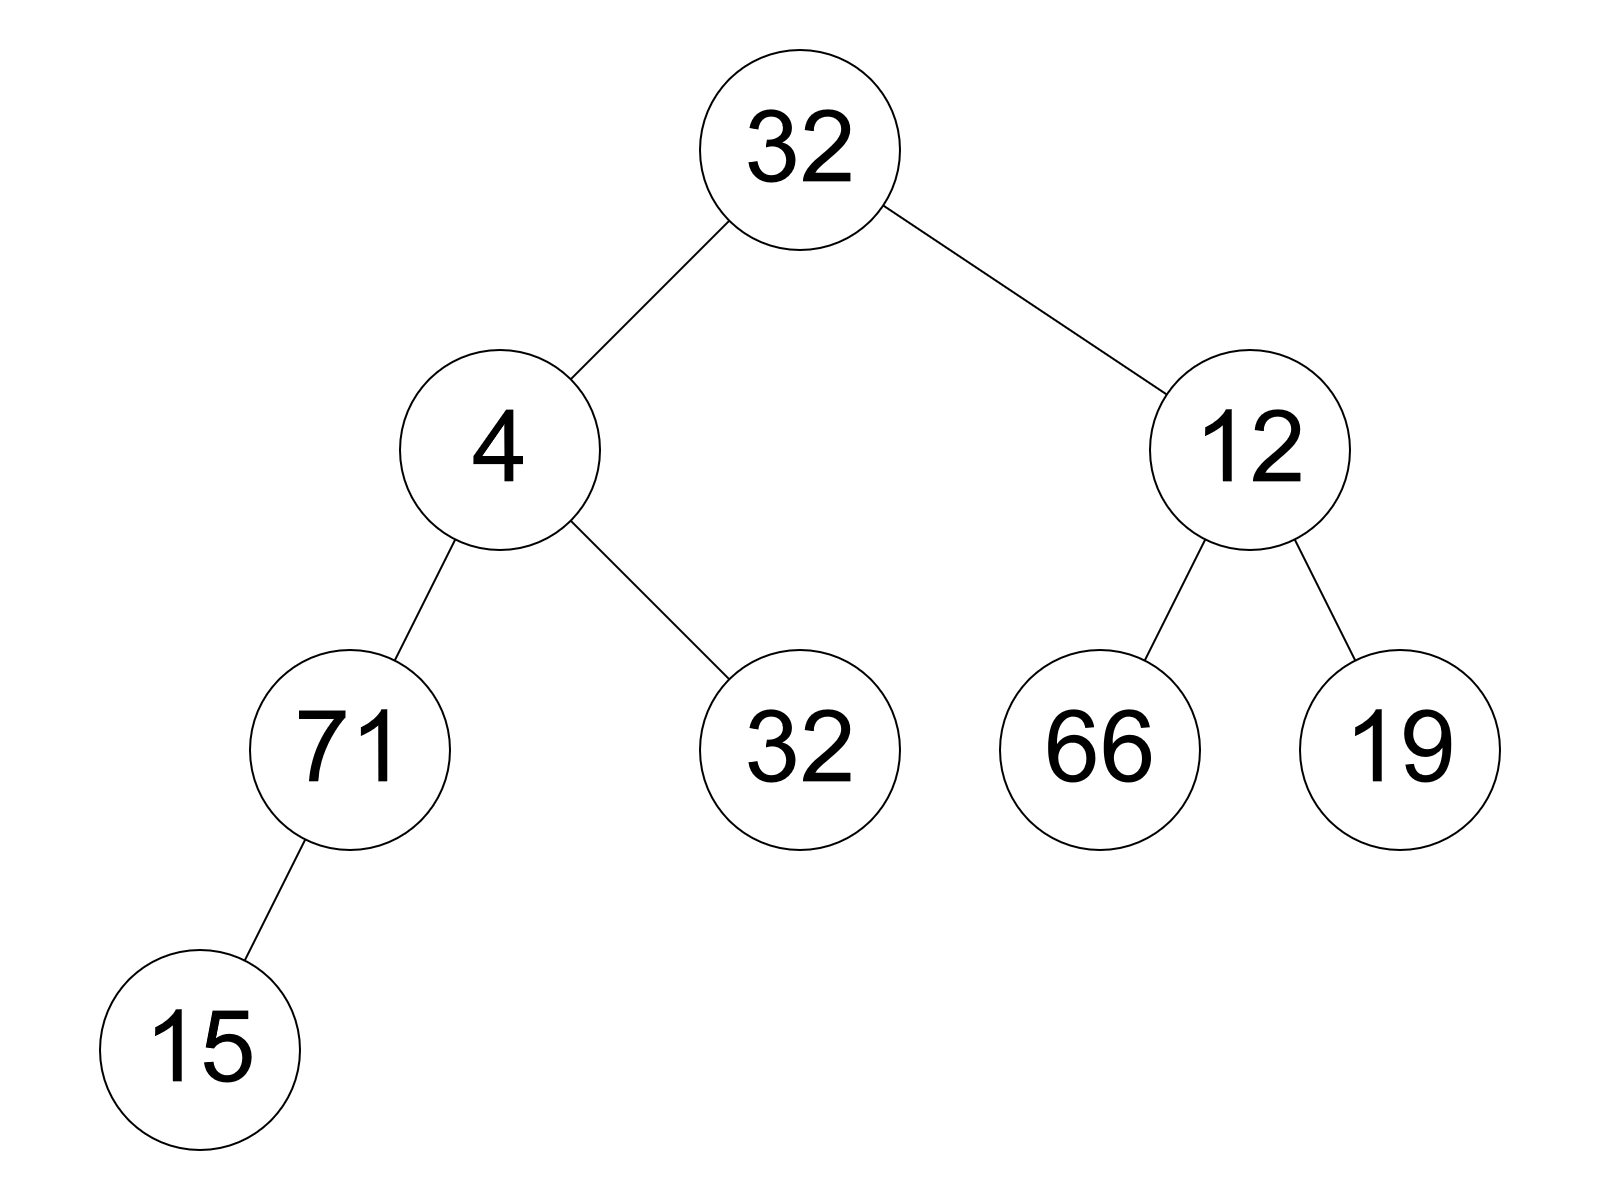
\includegraphics[width=\textwidth]{img/a1}
            \end{subfigure}
            \begin{subfigure}[b]{0.23\textwidth}
                \centering
                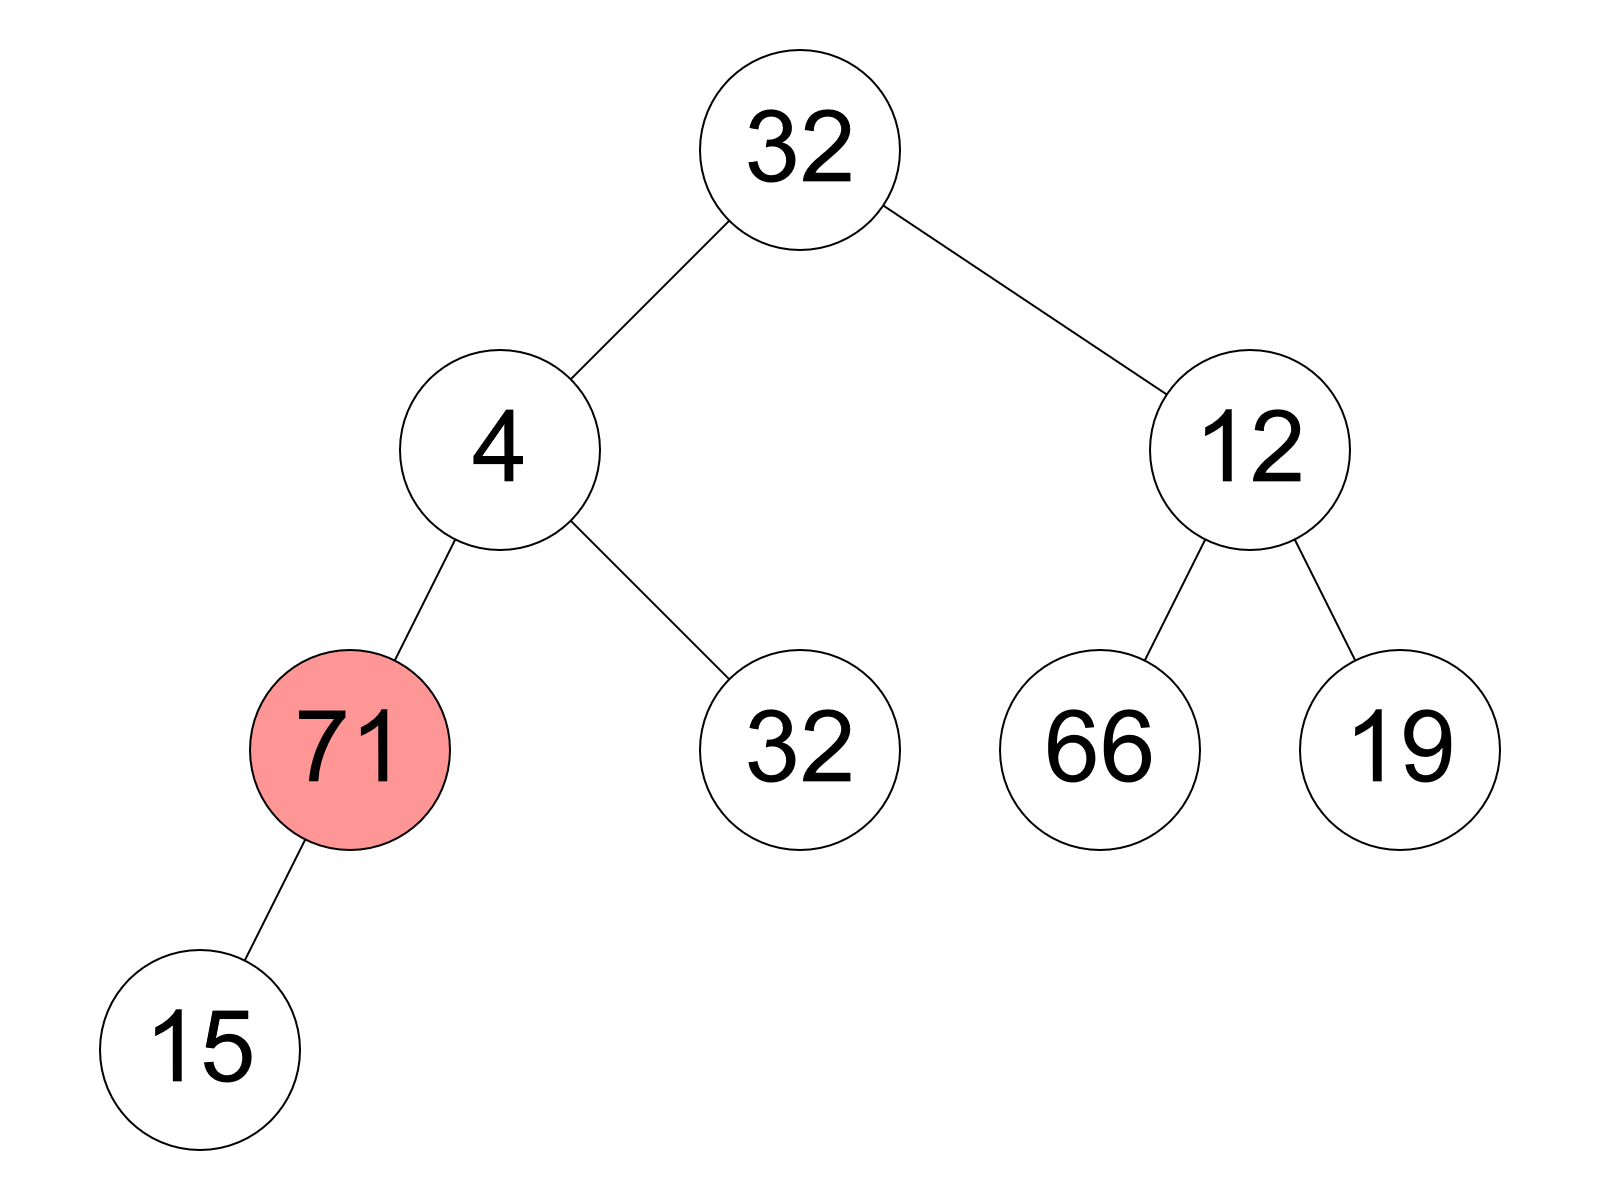
\includegraphics[width=\textwidth]{img/a2}
            \end{subfigure}
            \begin{subfigure}[b]{0.23\textwidth}
                \centering
                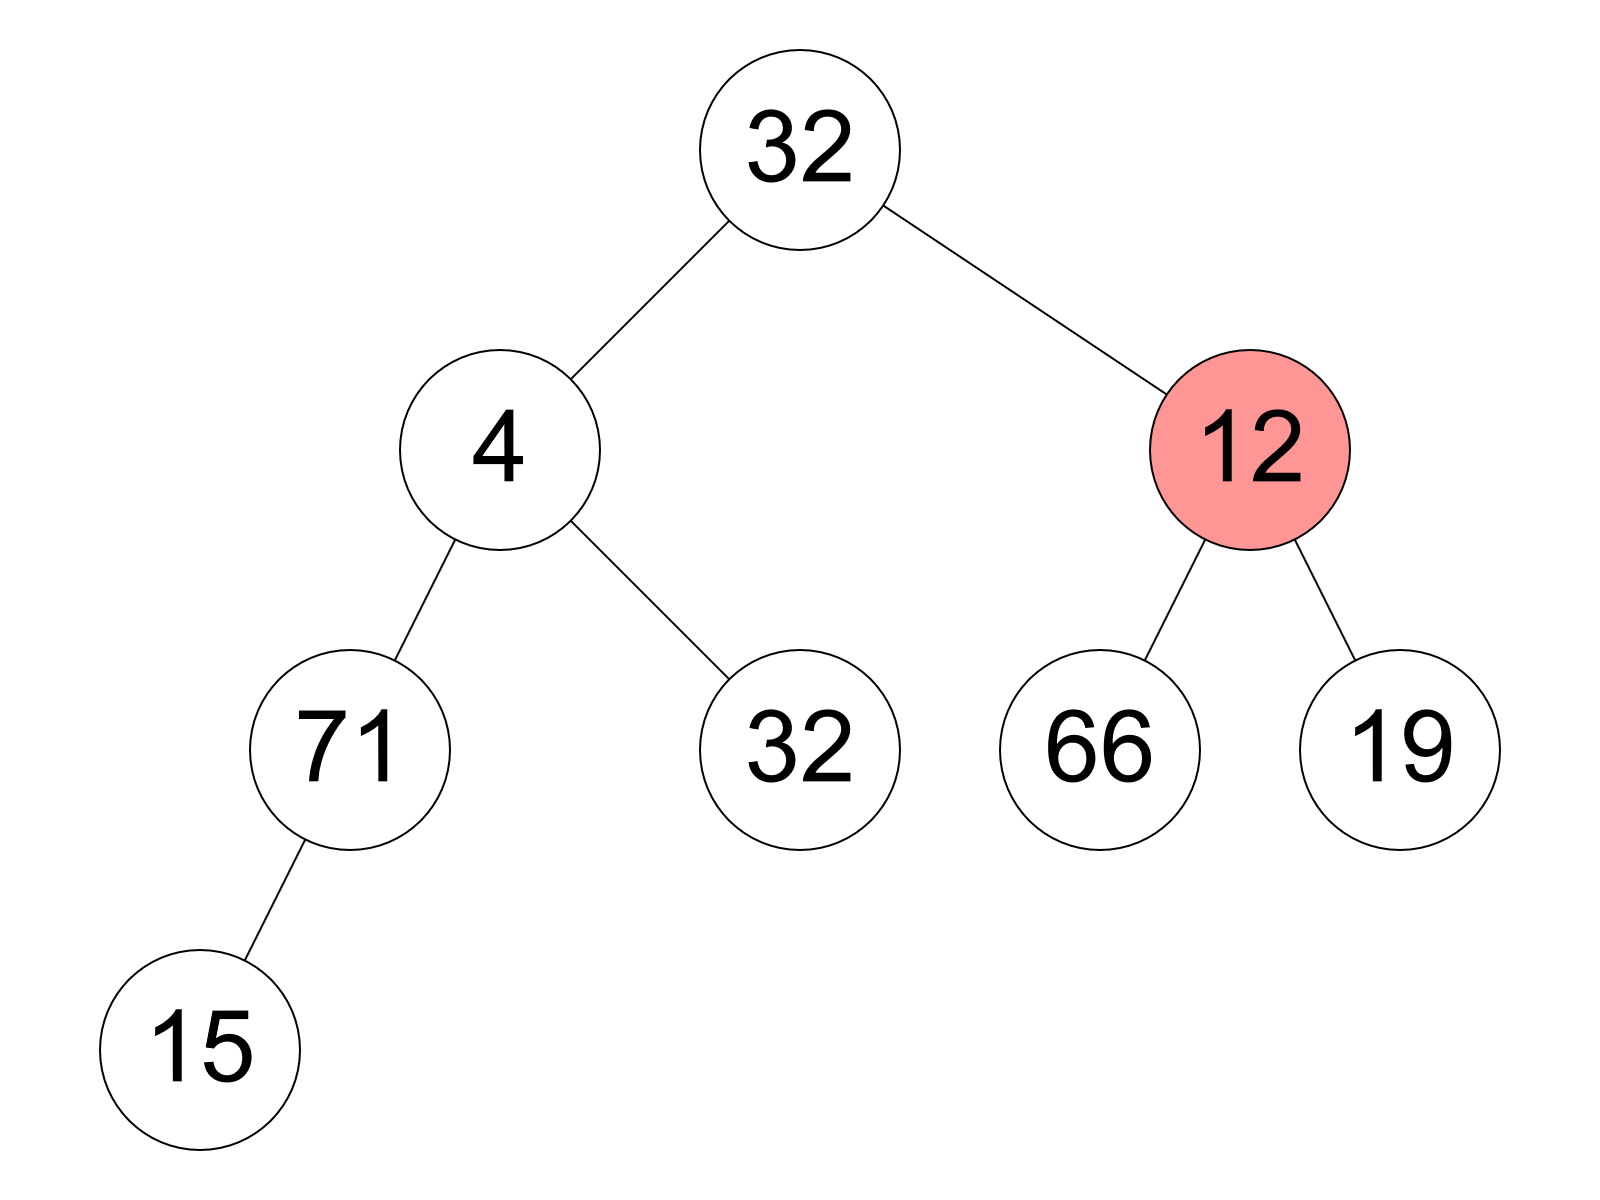
\includegraphics[width=\textwidth]{img/a3}
            \end{subfigure}
            \begin{subfigure}[b]{0.23\textwidth}
                \centering
                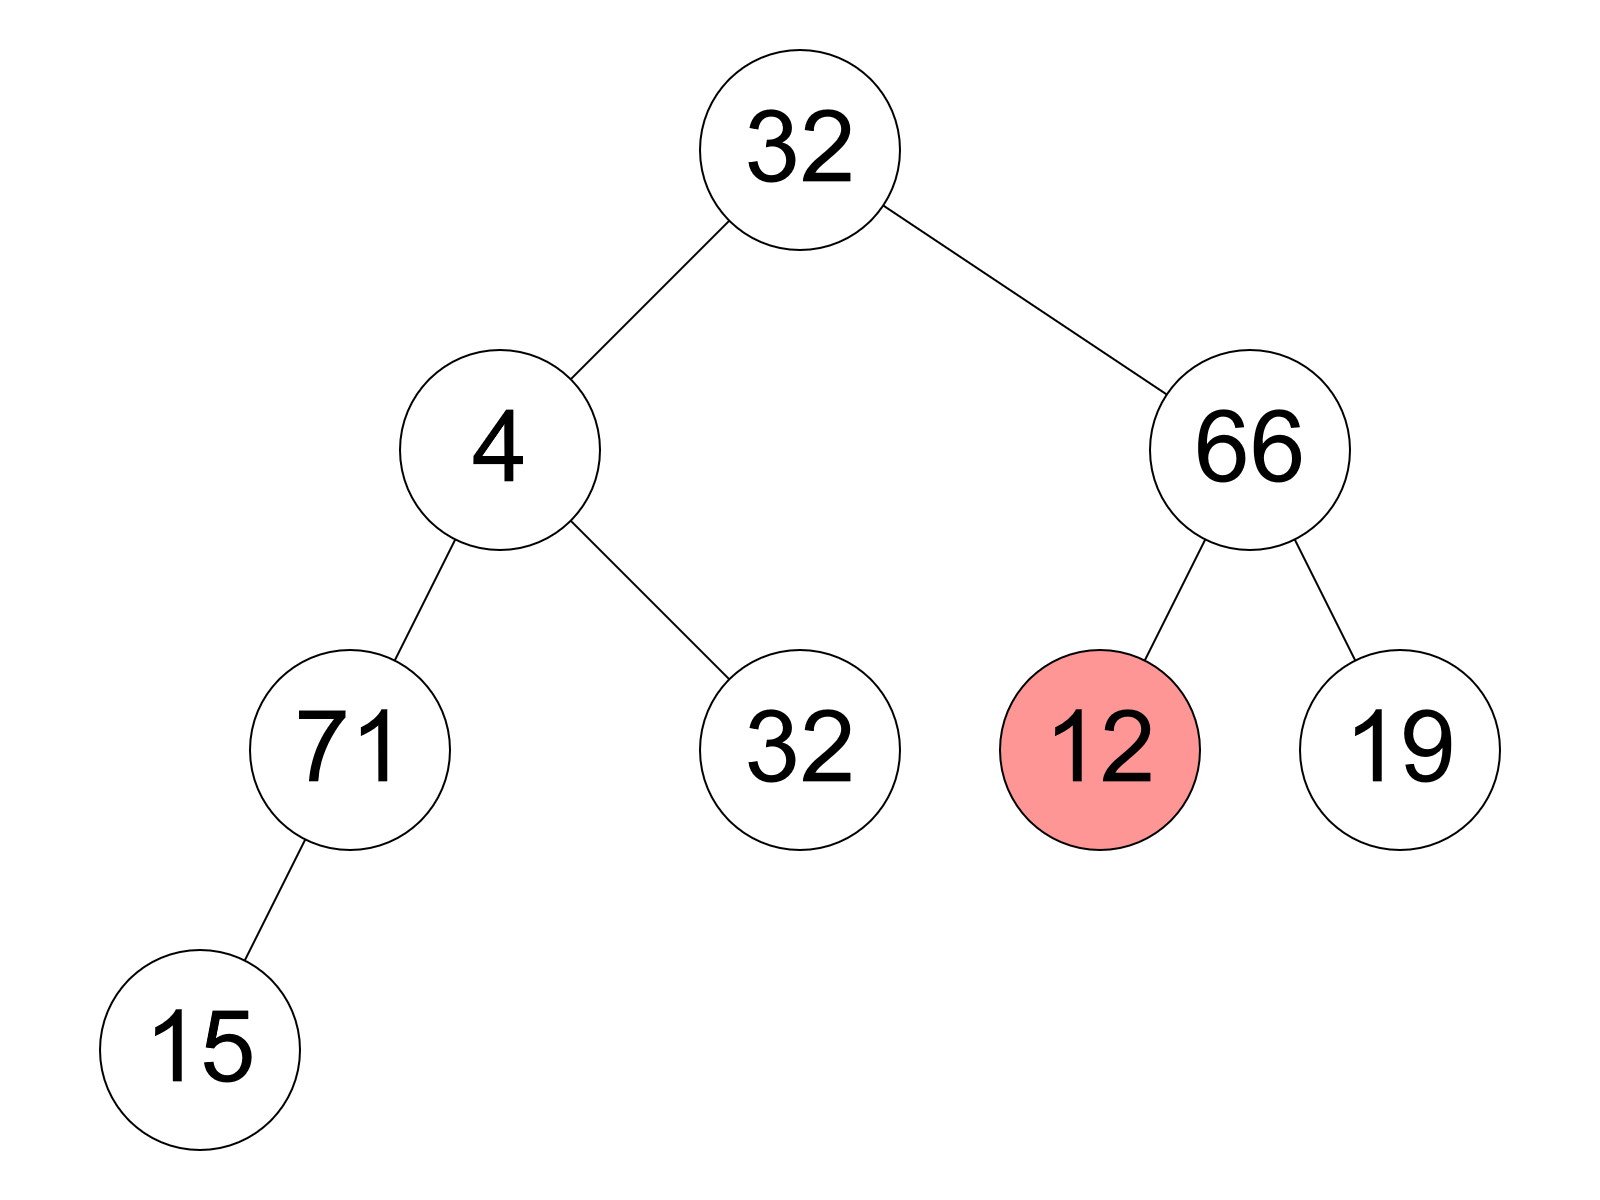
\includegraphics[width=\textwidth]{img/a4}
            \end{subfigure}
            \\
            \begin{subfigure}[b]{0.23\textwidth}
                \centering
                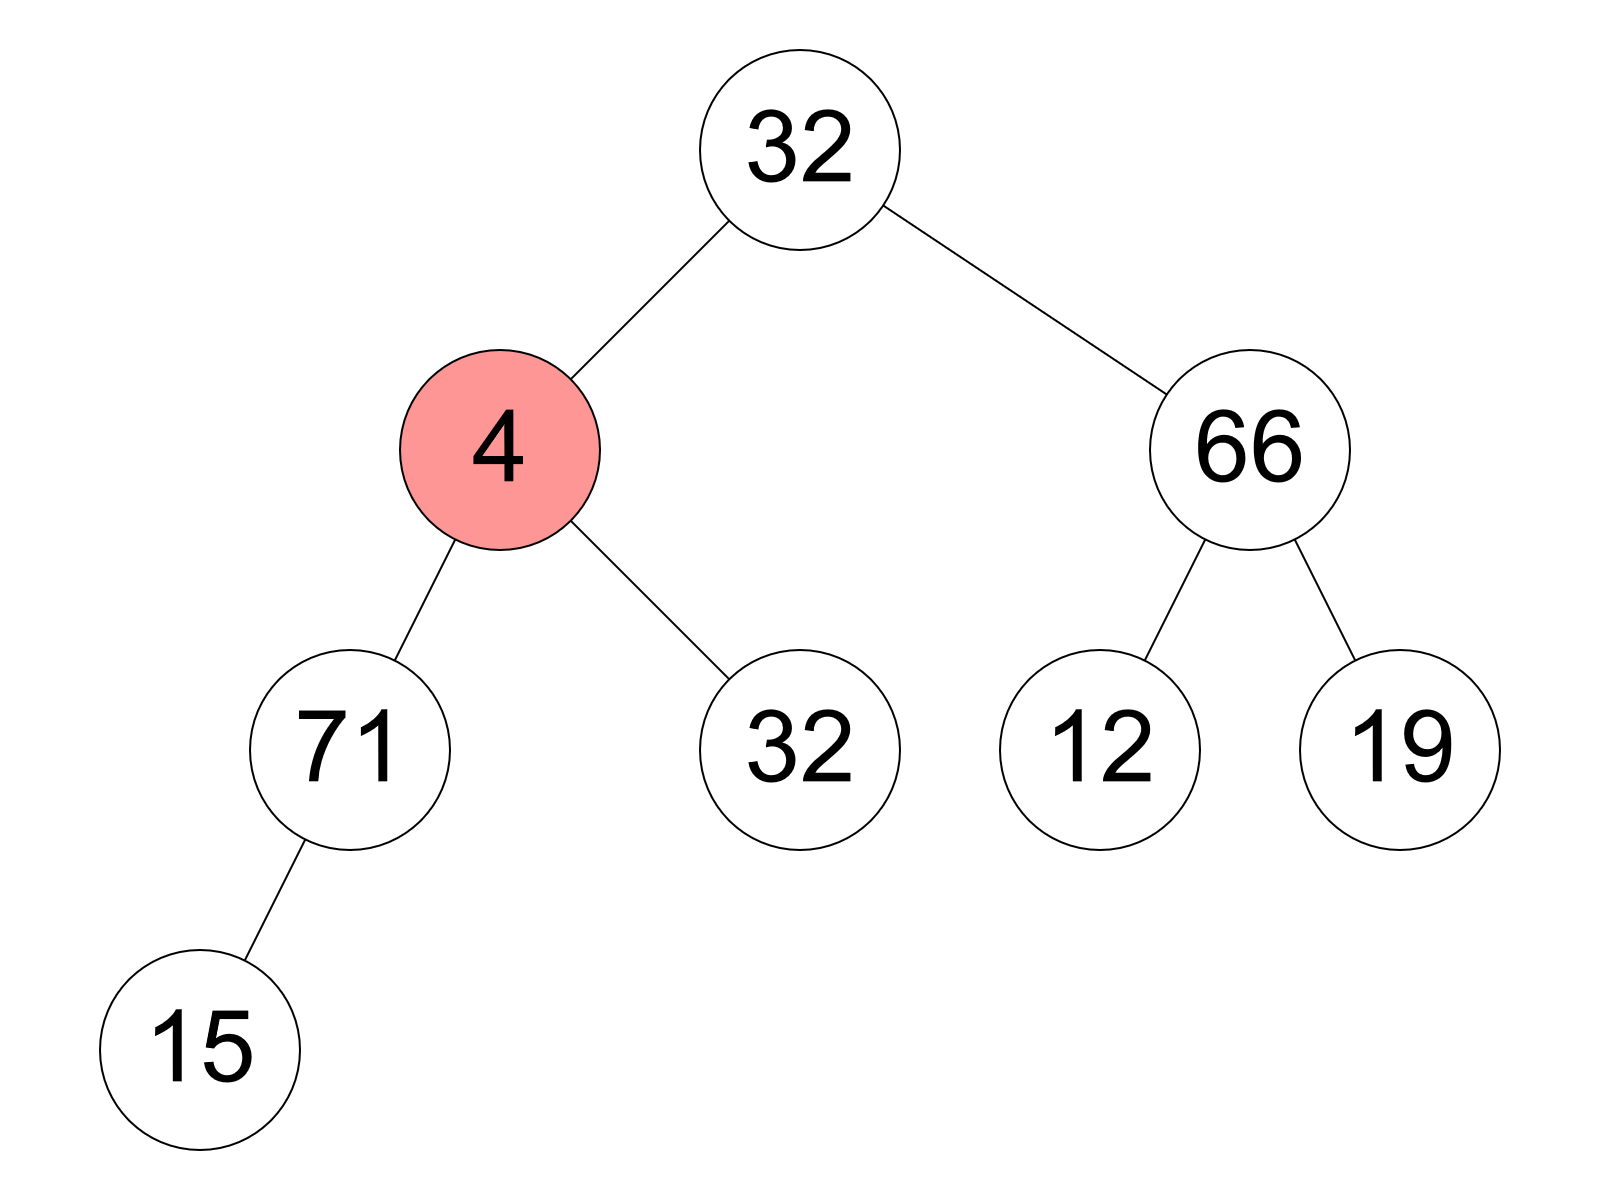
\includegraphics[width=\textwidth]{img/a5}
            \end{subfigure}
            \begin{subfigure}[b]{0.23\textwidth}
                \centering
                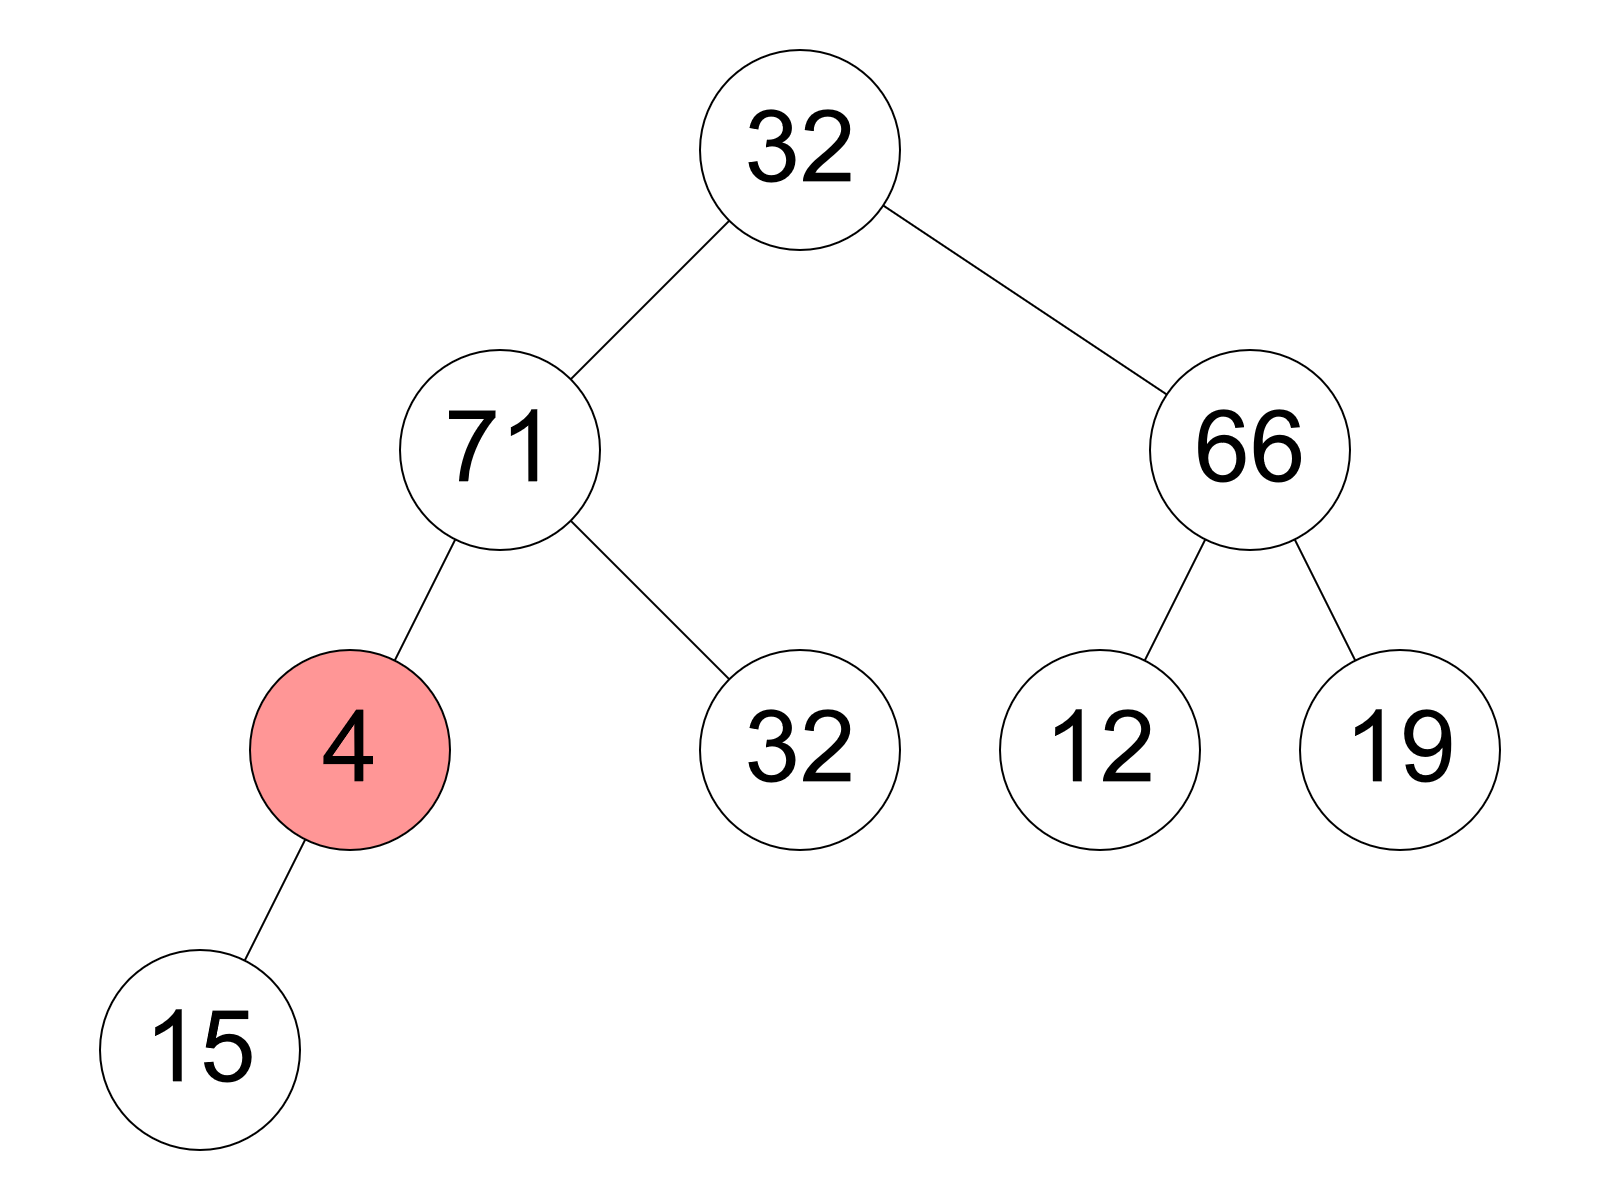
\includegraphics[width=\textwidth]{img/a6}
            \end{subfigure}
            \begin{subfigure}[b]{0.23\textwidth}
                \centering
                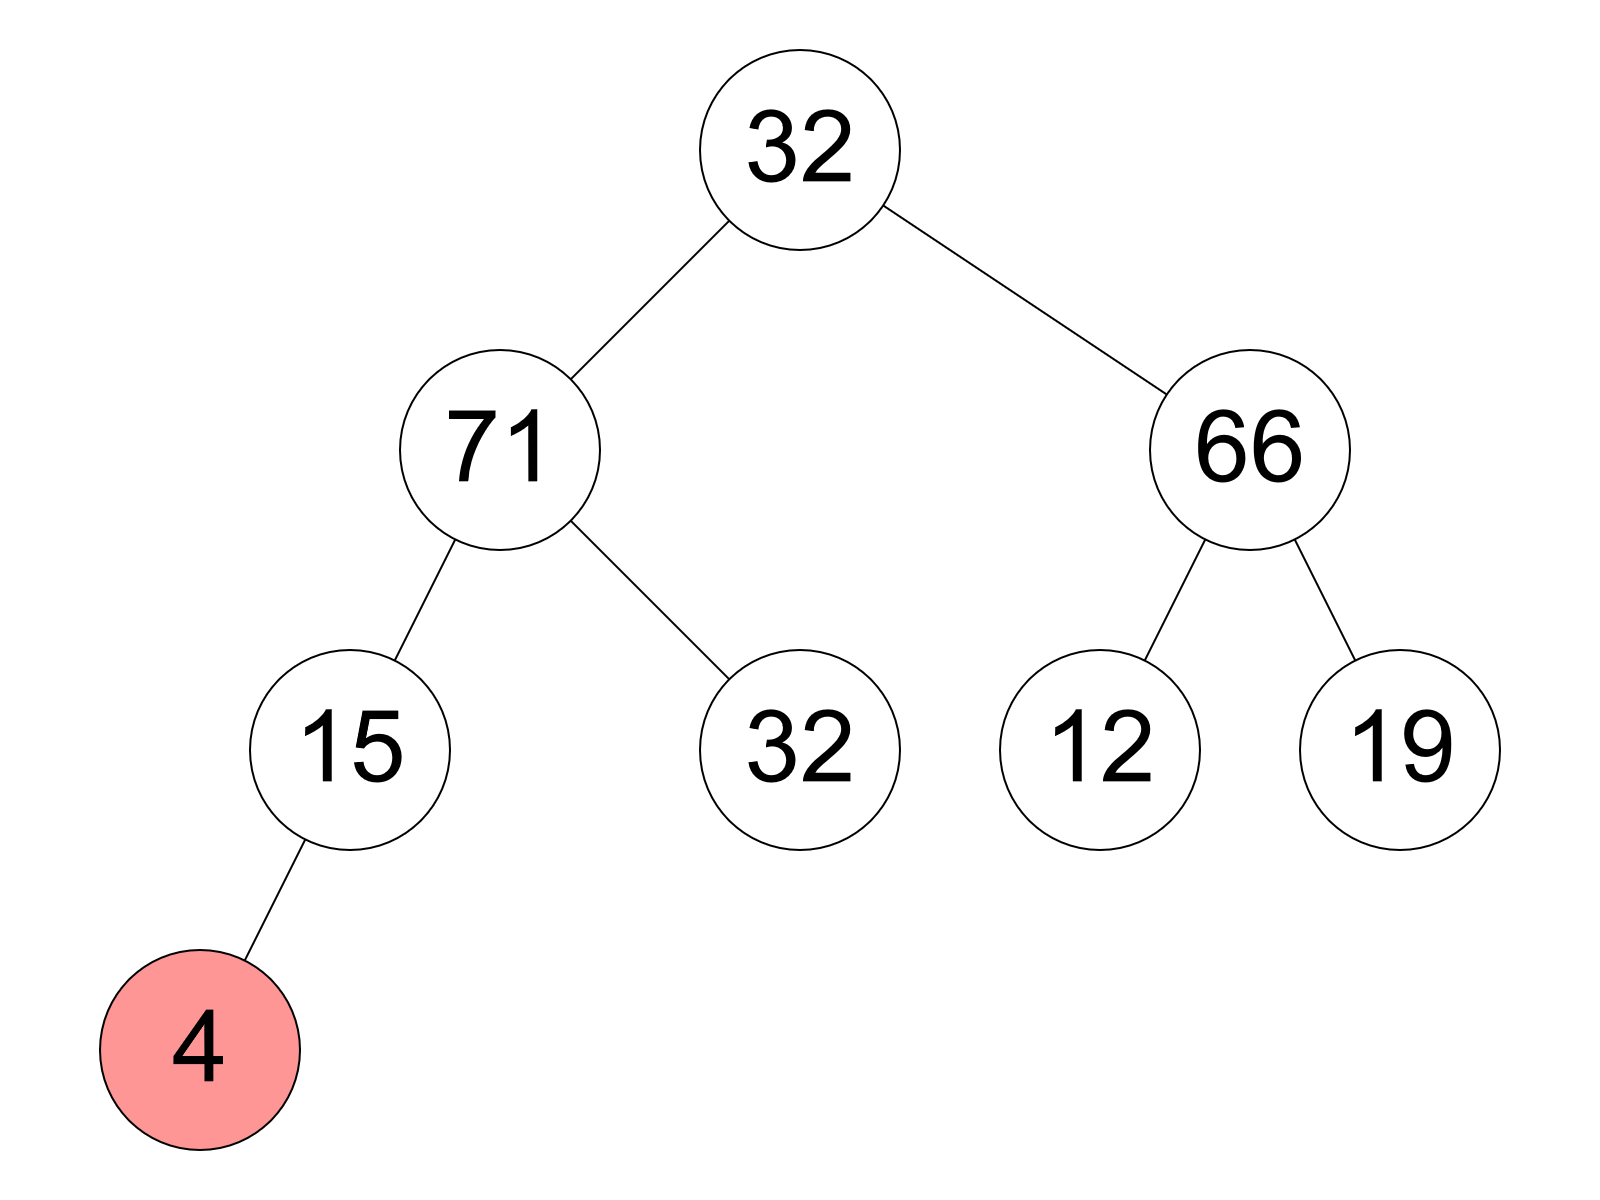
\includegraphics[width=\textwidth]{img/a8}
            \end{subfigure}
            \\
            \begin{subfigure}[b]{0.23\textwidth}
                \centering
                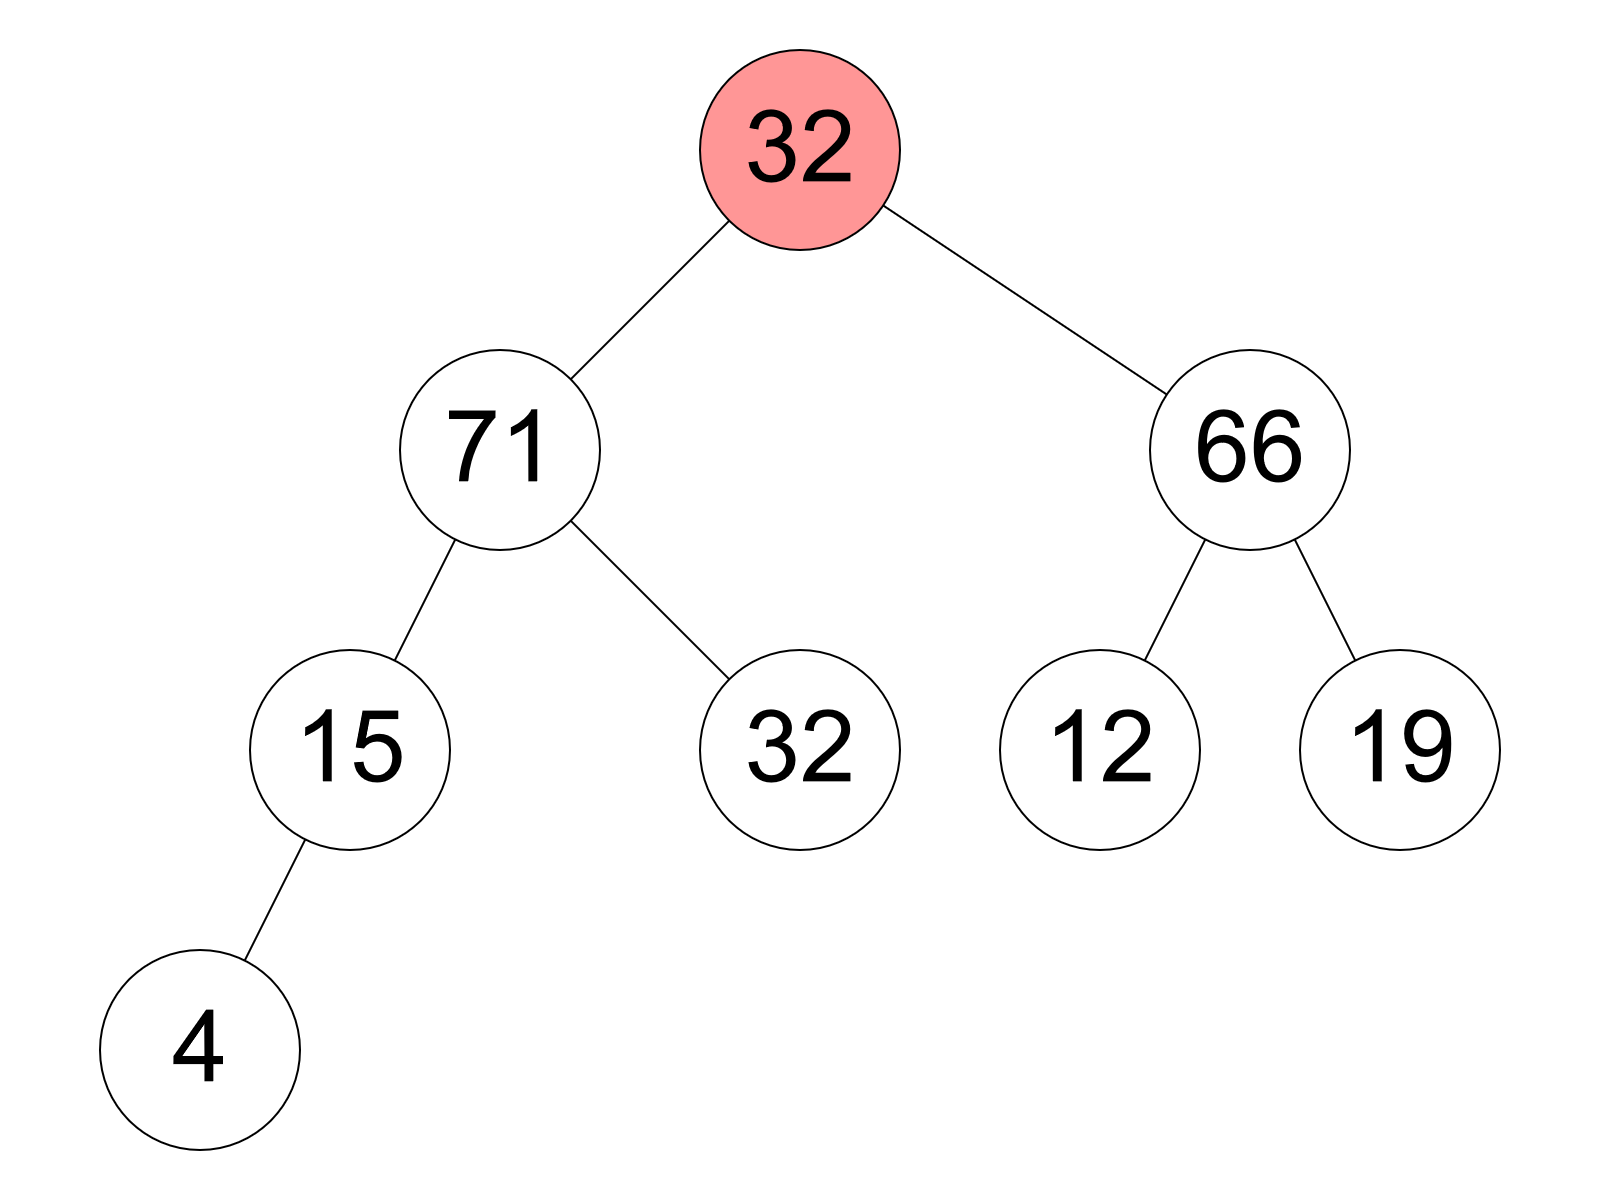
\includegraphics[width=\textwidth]{img/a9}
            \end{subfigure}
            \begin{subfigure}[b]{0.23\textwidth}
                \centering
                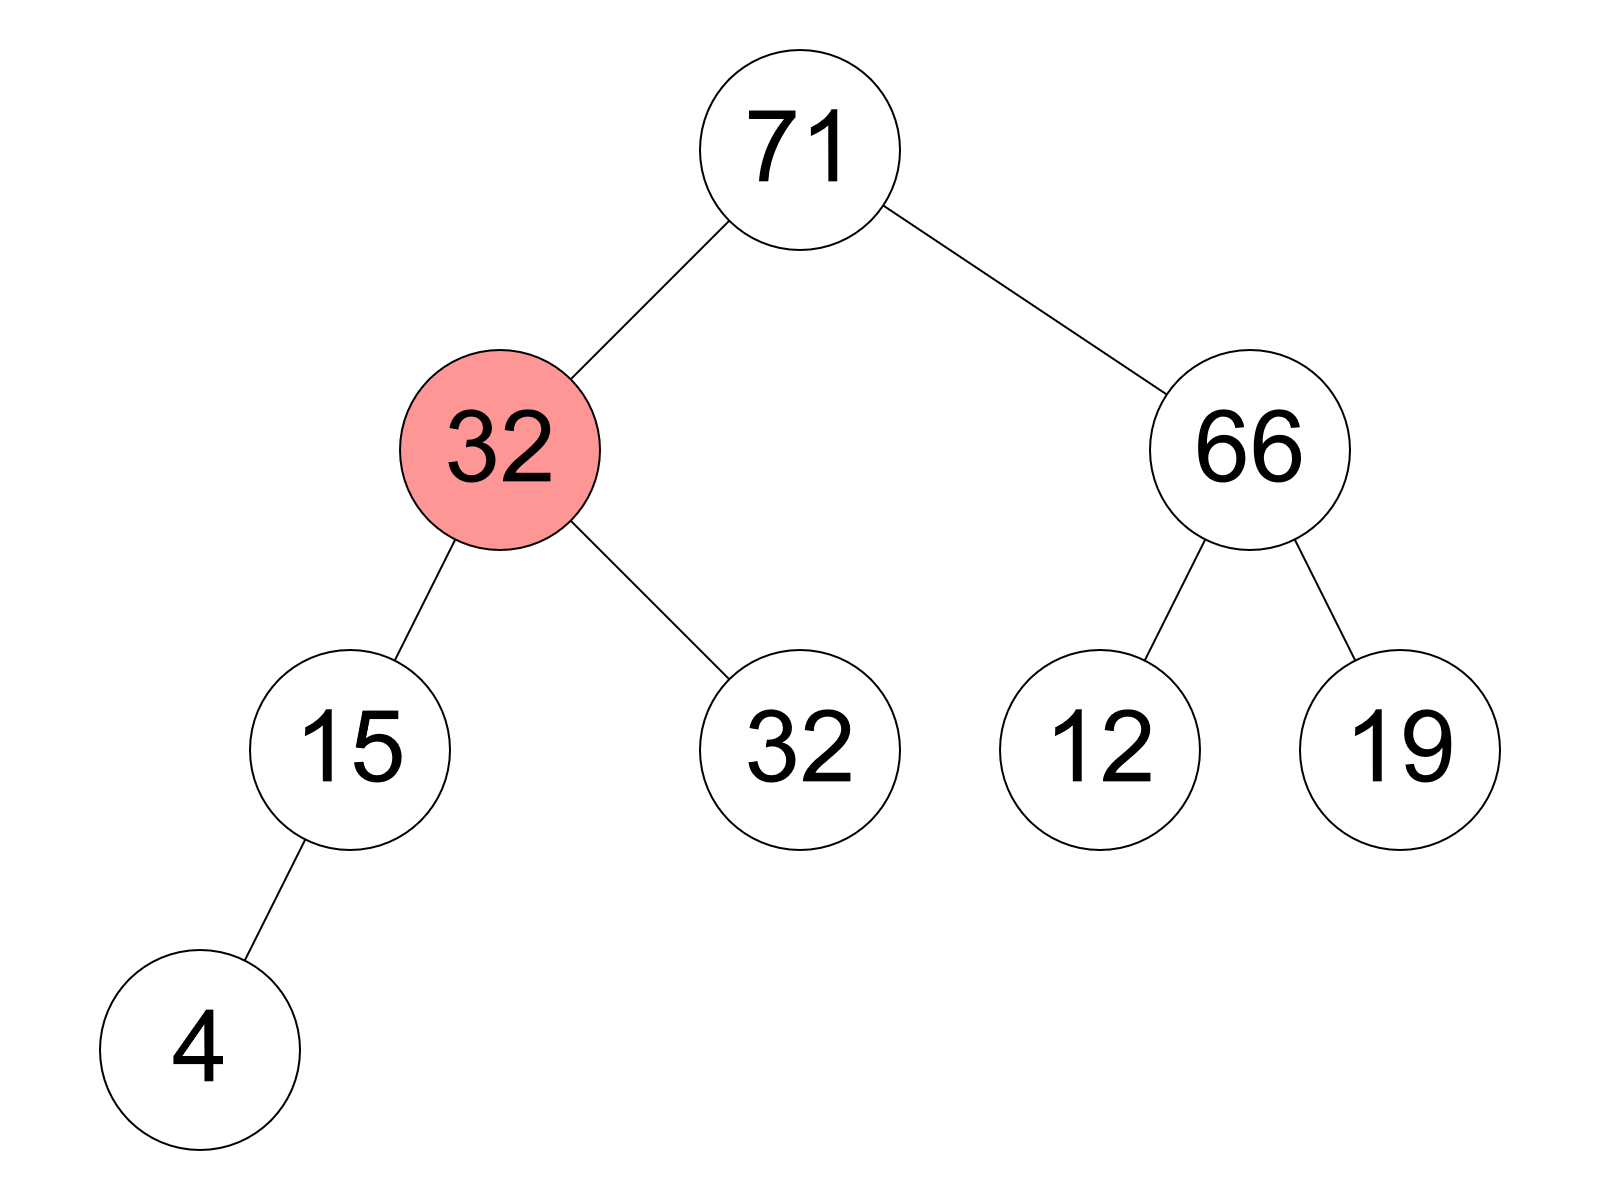
\includegraphics[width=\textwidth]{img/a10}
            \end{subfigure}
        \end{figure}
        \FloatBarrier

        \item \ \\
        \begin{figure}[h!]
            \centering
            \begin{subfigure}[b]{0.23\textwidth}
                \centering
                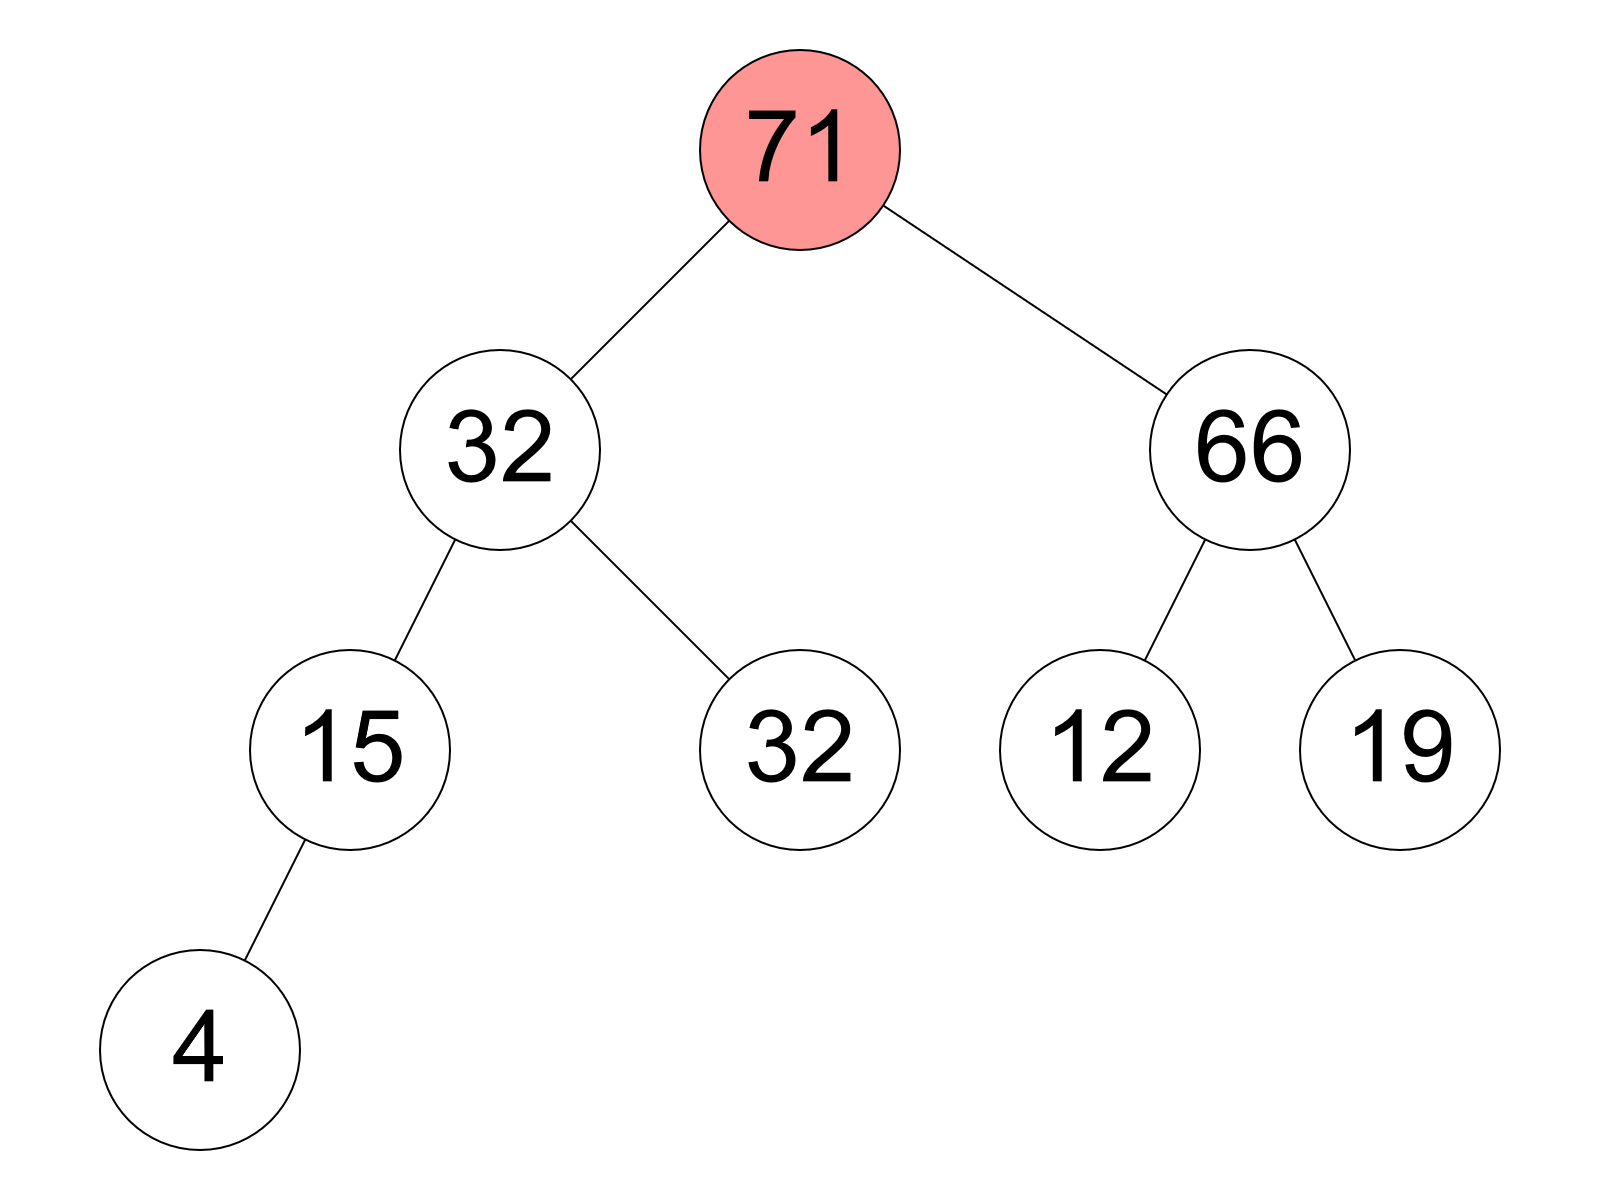
\includegraphics[width=\textwidth]{img/b1}
            \end{subfigure}
            \begin{subfigure}[b]{0.23\textwidth}
                \centering
                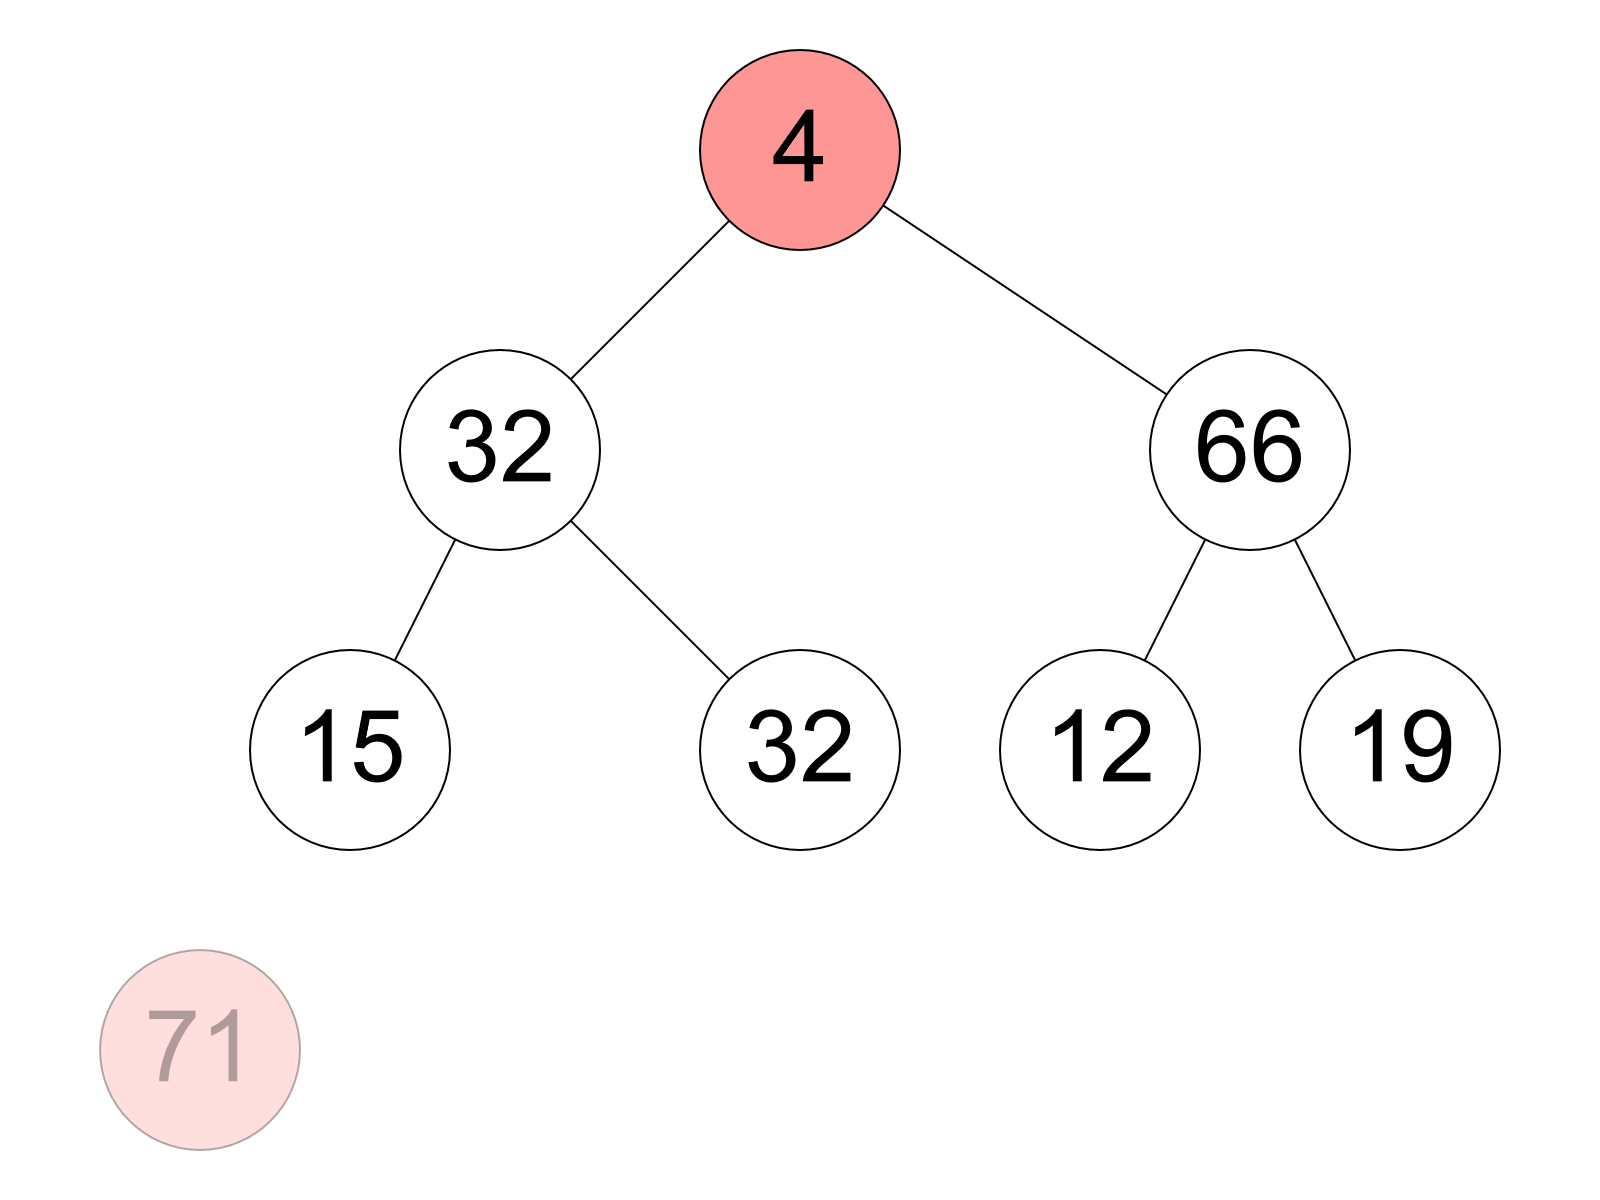
\includegraphics[width=\textwidth]{img/b2}
            \end{subfigure}
            \begin{subfigure}[b]{0.23\textwidth}
                \centering
                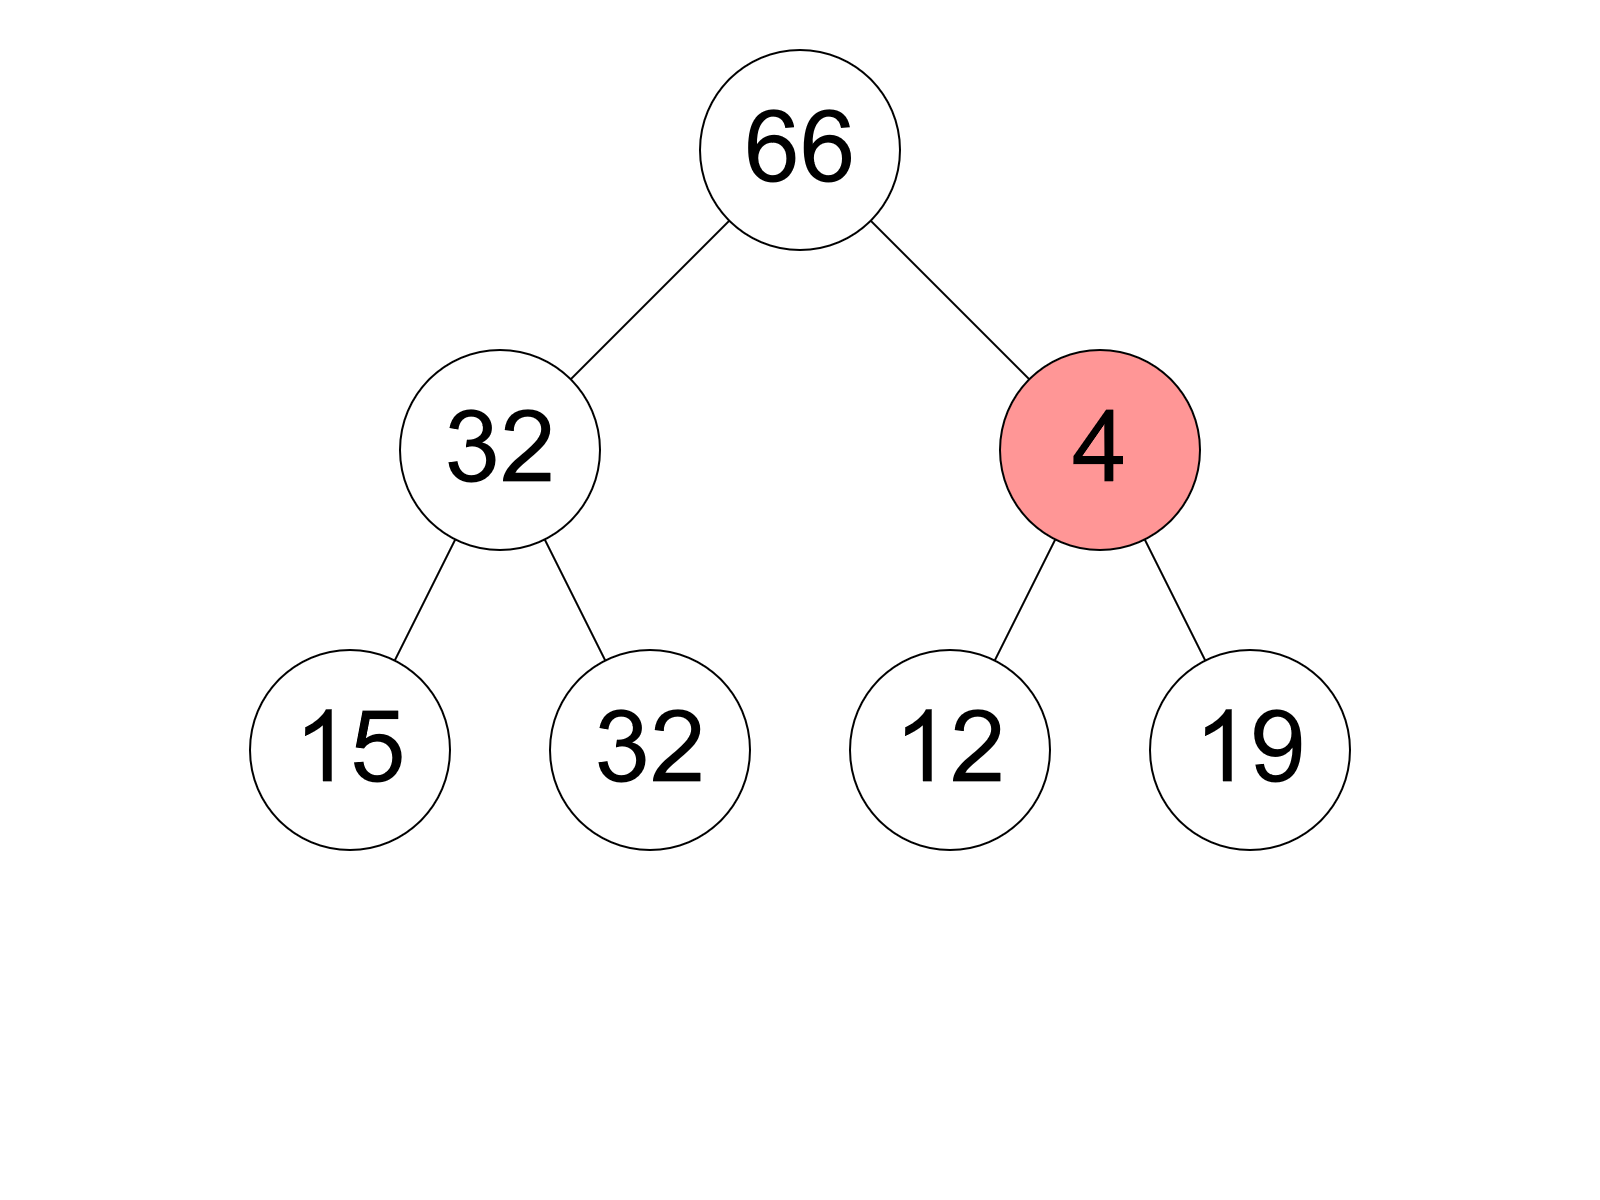
\includegraphics[width=\textwidth]{img/b3}
            \end{subfigure}
            \begin{subfigure}[b]{0.23\textwidth}
                \centering
                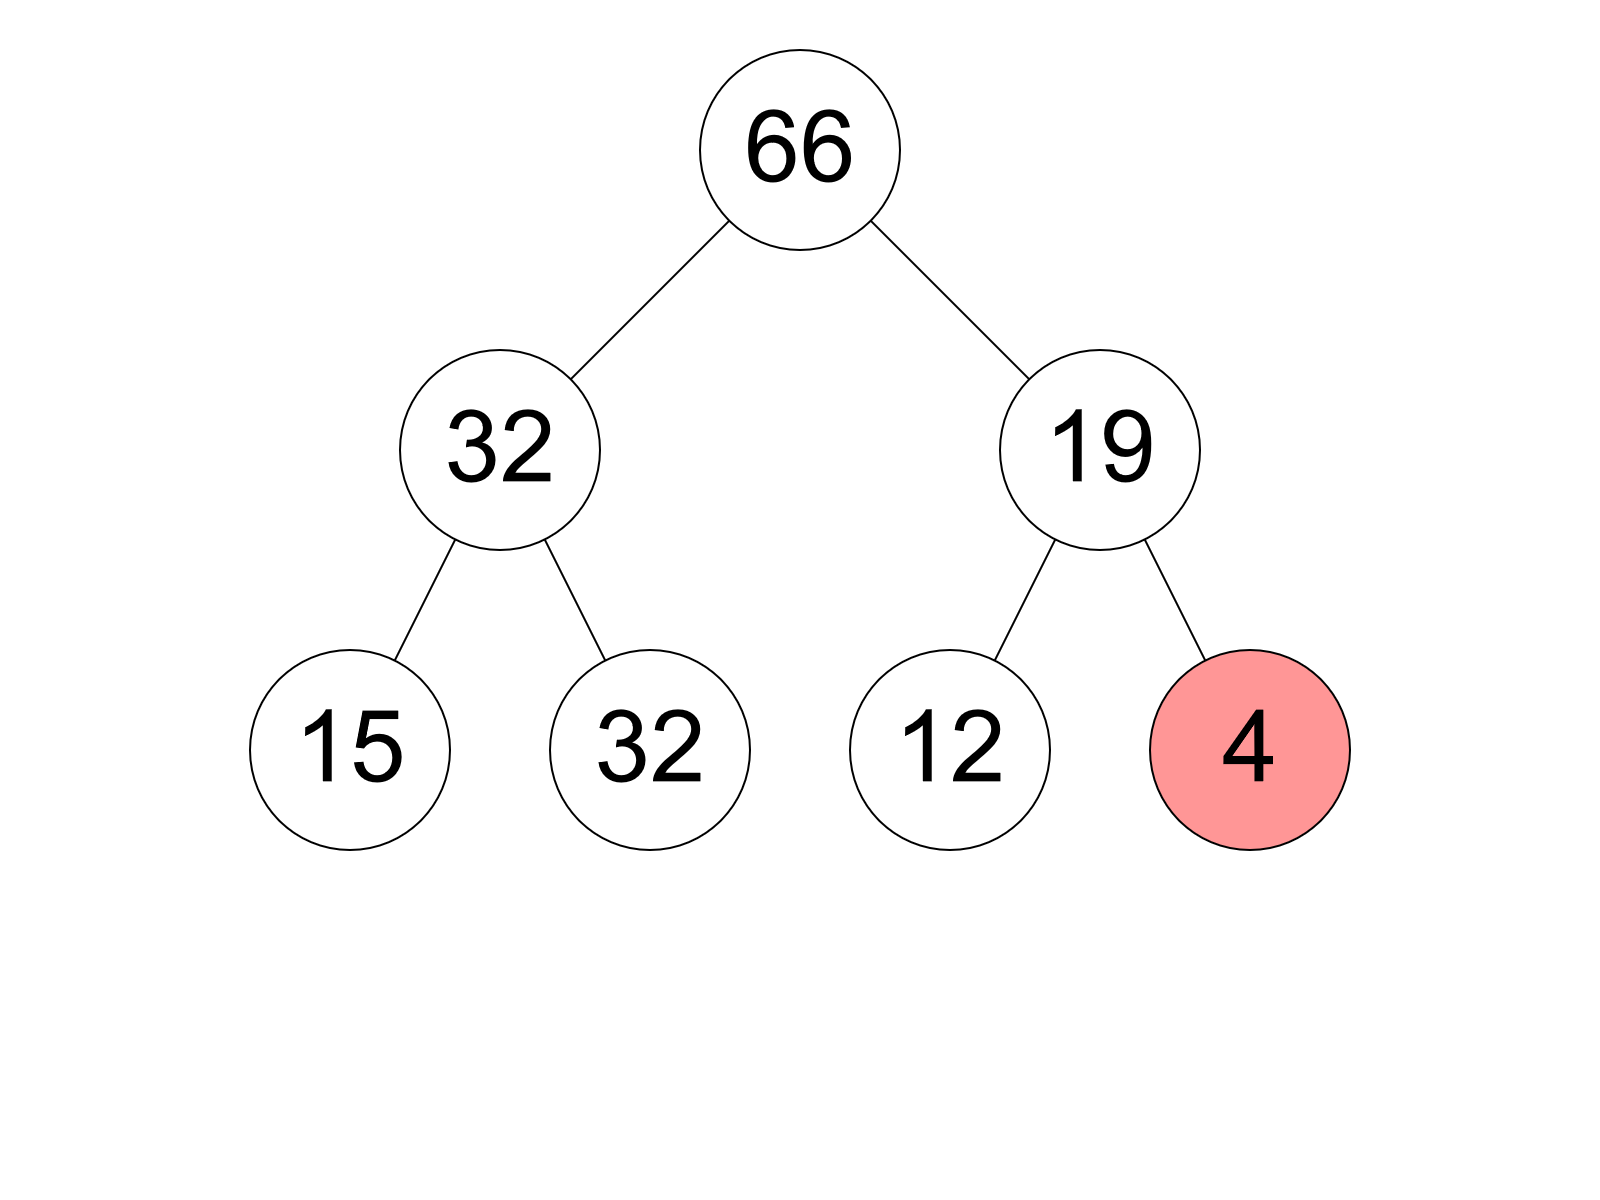
\includegraphics[width=\textwidth]{img/b5}
            \end{subfigure}
            \\
            \begin{subfigure}[b]{0.23\textwidth}
                \centering
                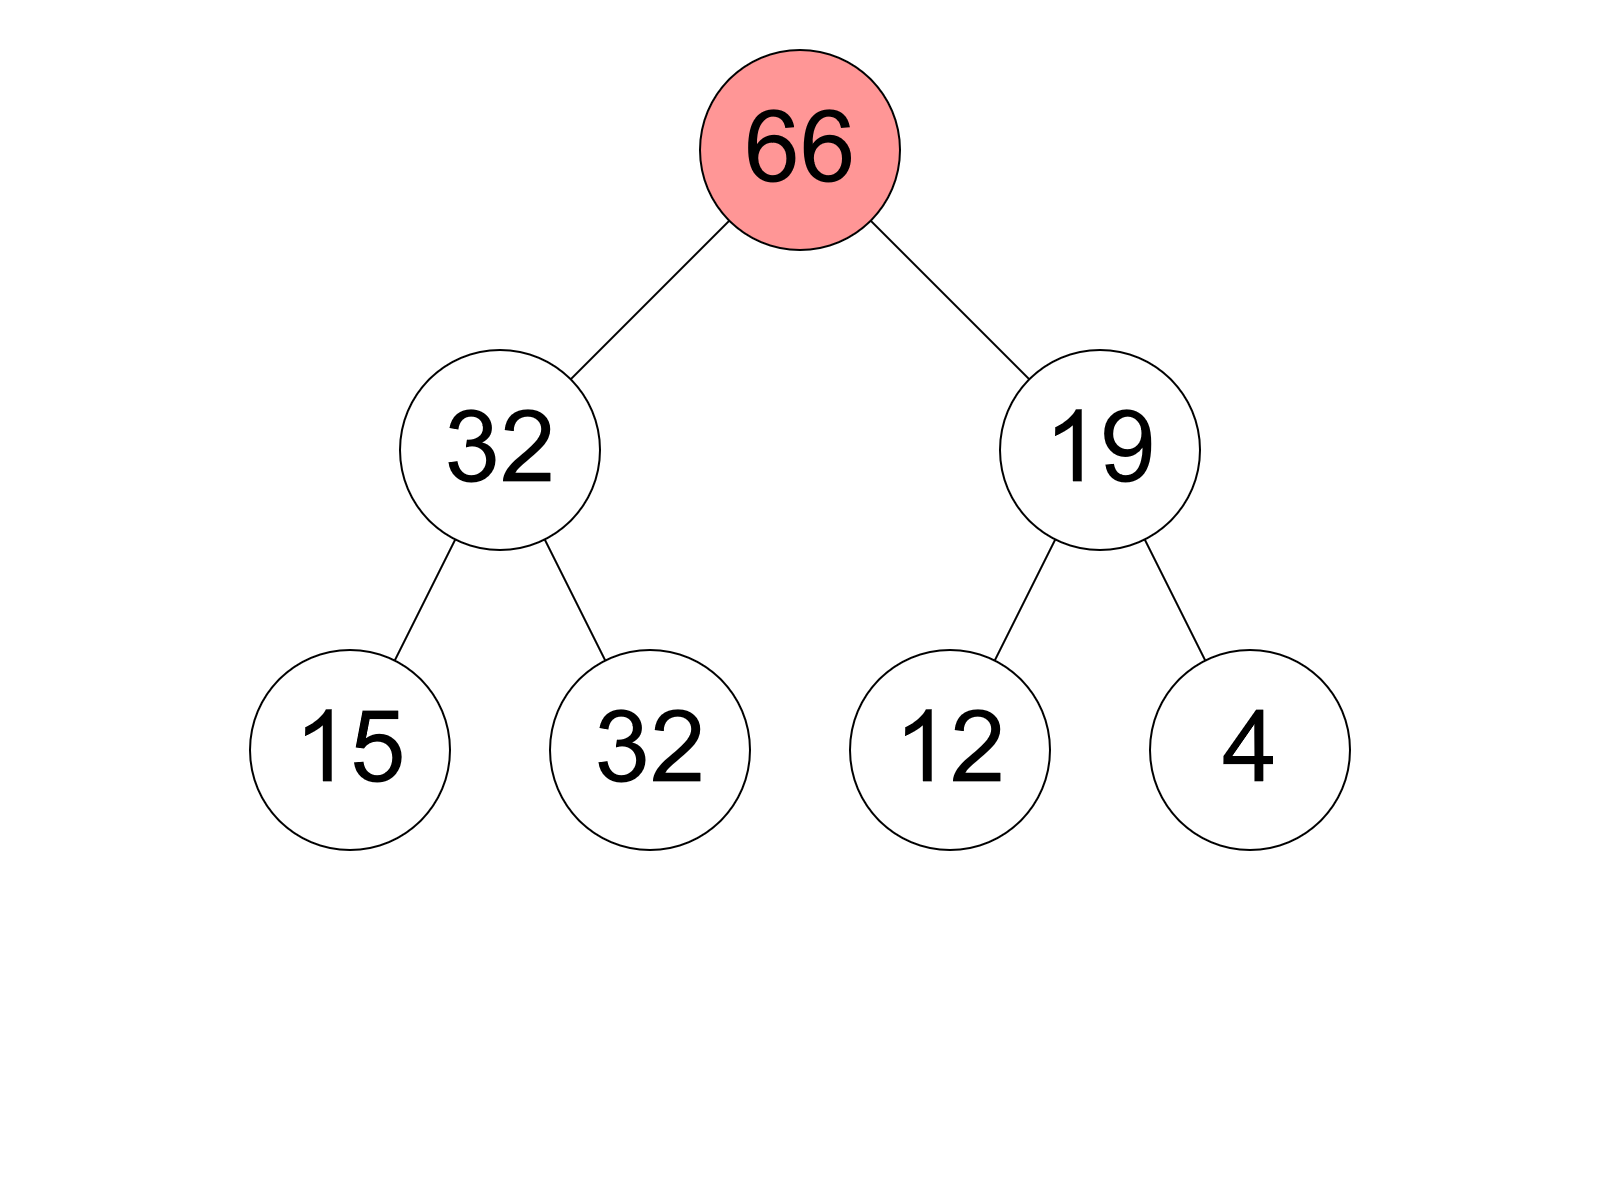
\includegraphics[width=\textwidth]{img/b6}
            \end{subfigure}
            \begin{subfigure}[b]{0.23\textwidth}
                \centering
                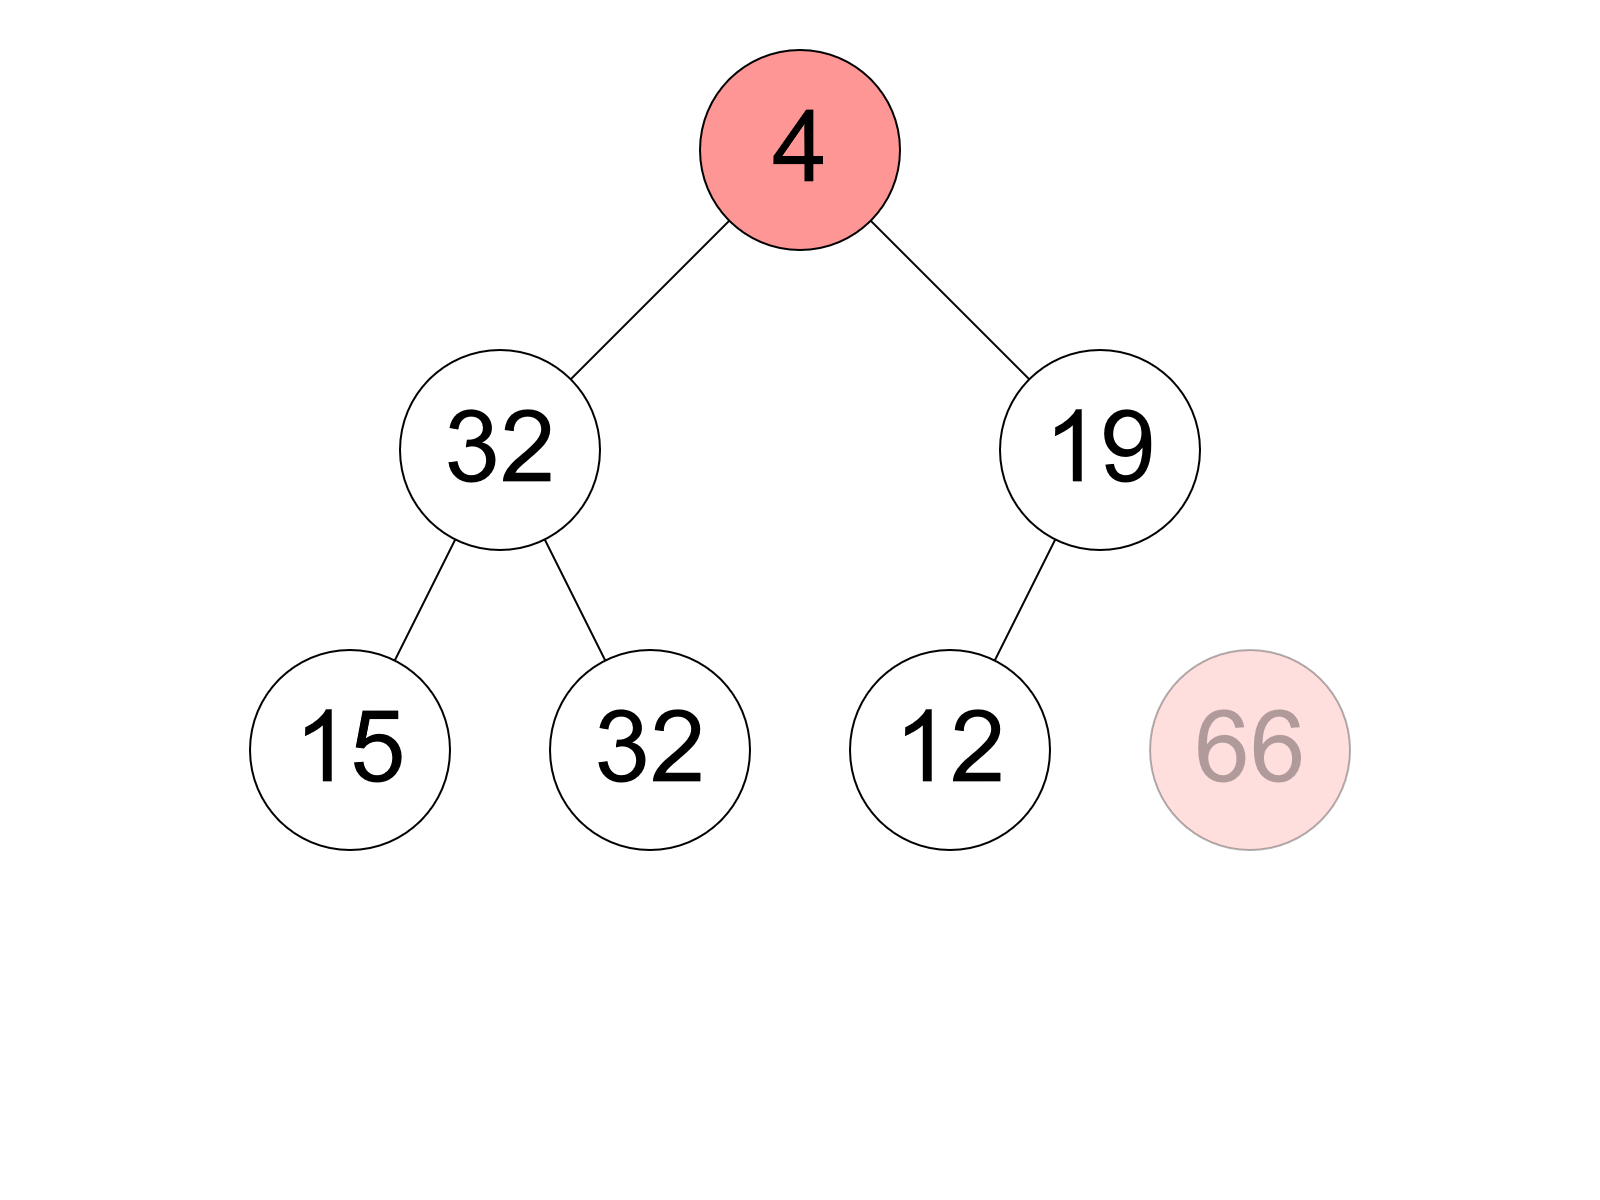
\includegraphics[width=\textwidth]{img/b7}
            \end{subfigure}
            \begin{subfigure}[b]{0.23\textwidth}
                \centering
                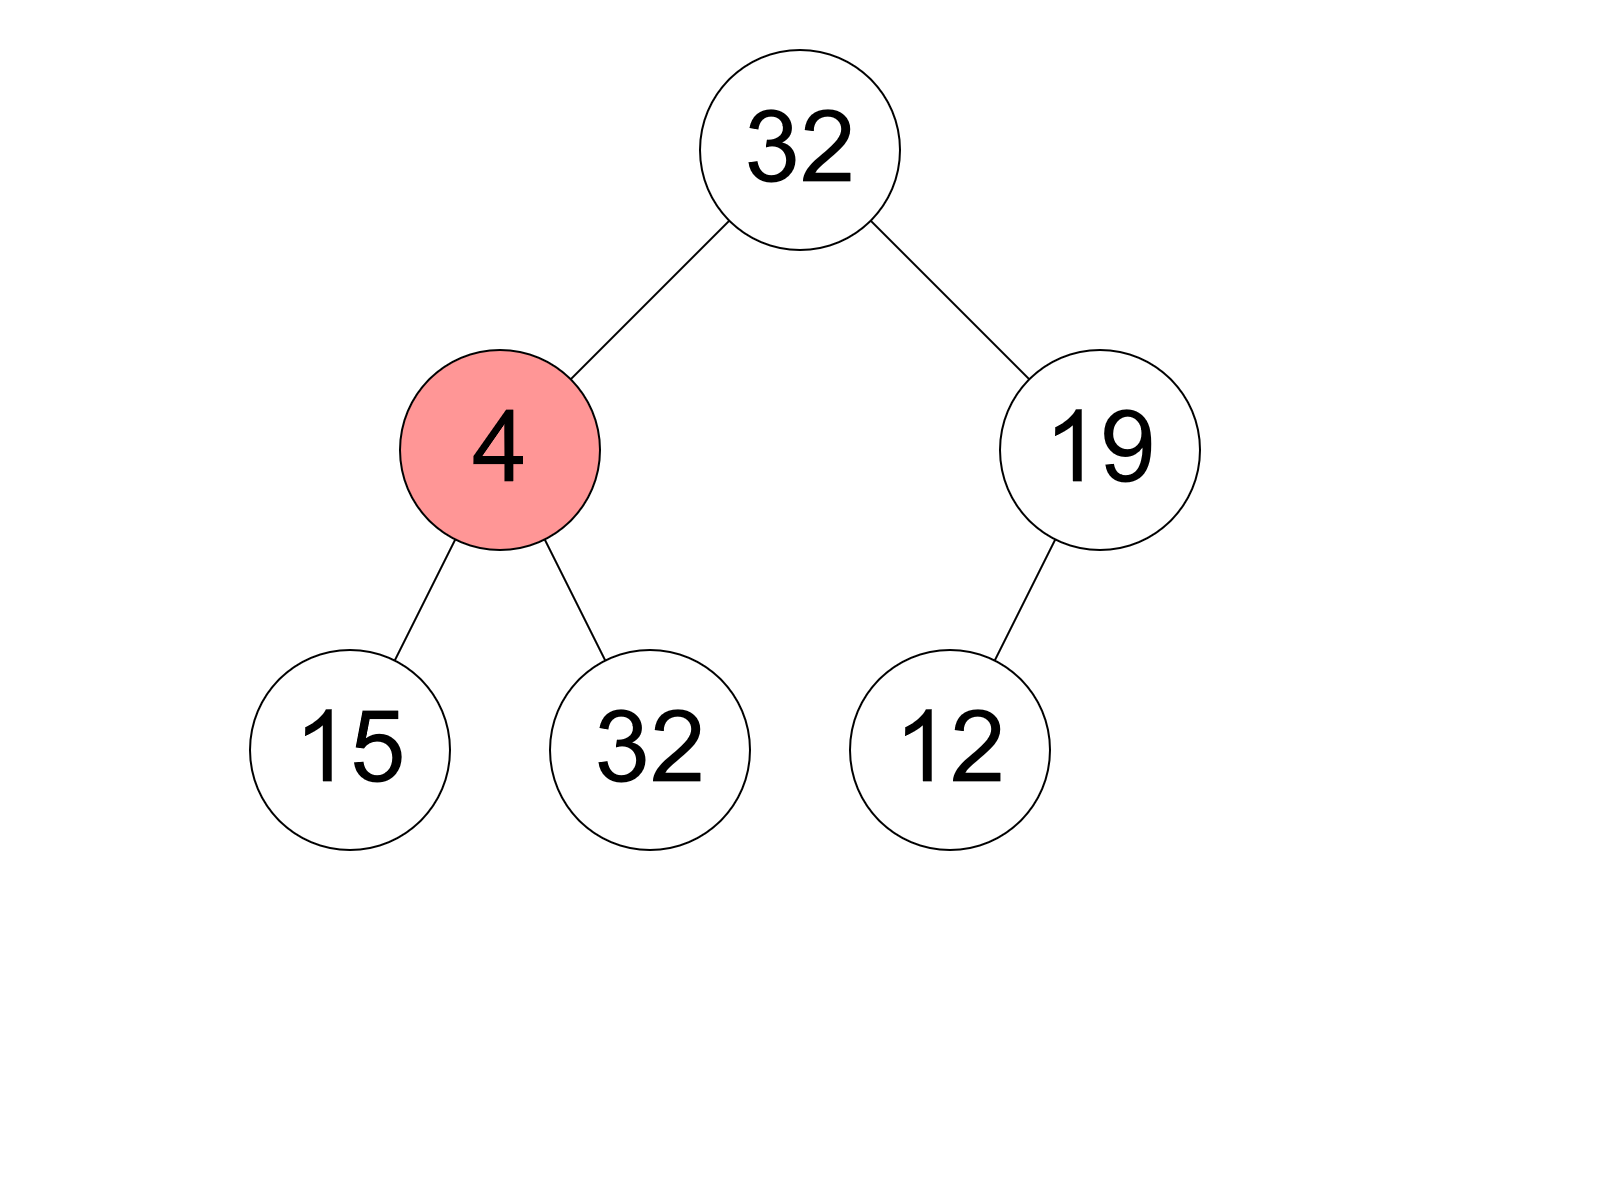
\includegraphics[width=\textwidth]{img/b8}
            \end{subfigure}
            \begin{subfigure}[b]{0.23\textwidth}
                \centering
                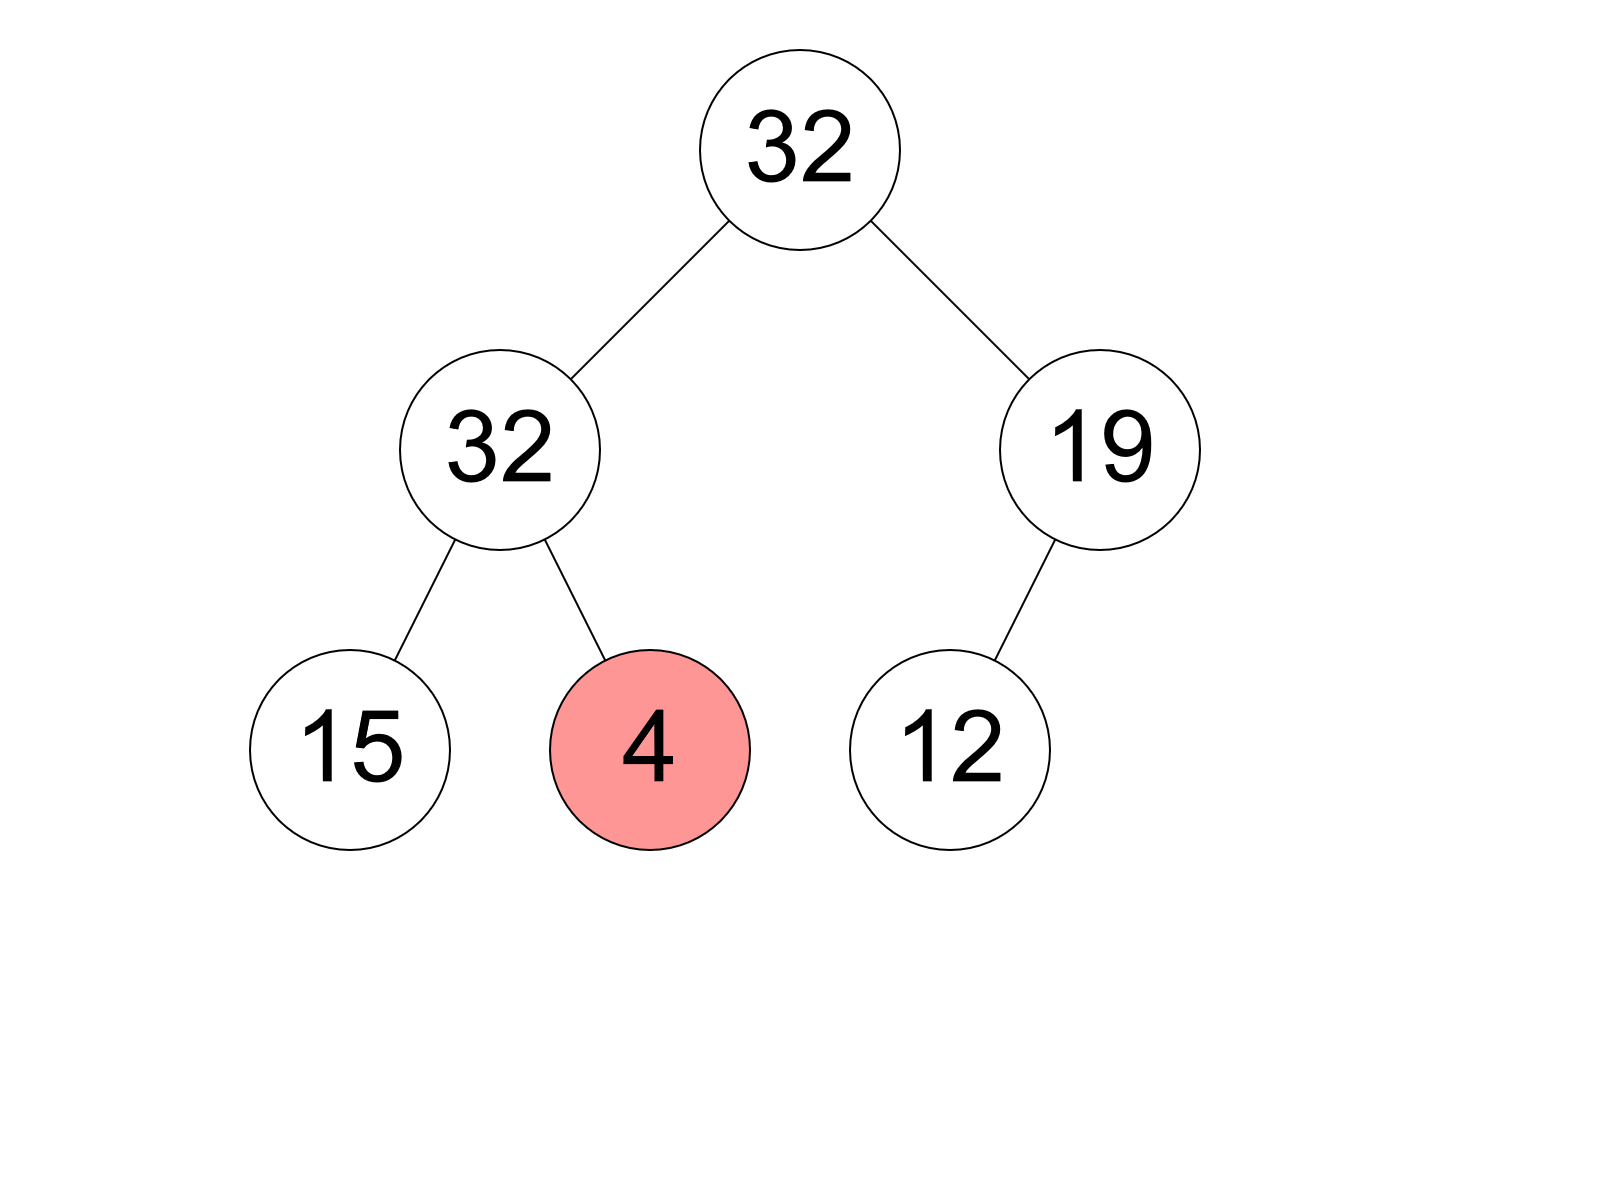
\includegraphics[width=\textwidth]{img/b9}
            \end{subfigure}
            \\
            \begin{subfigure}[b]{0.23\textwidth}
                \centering
                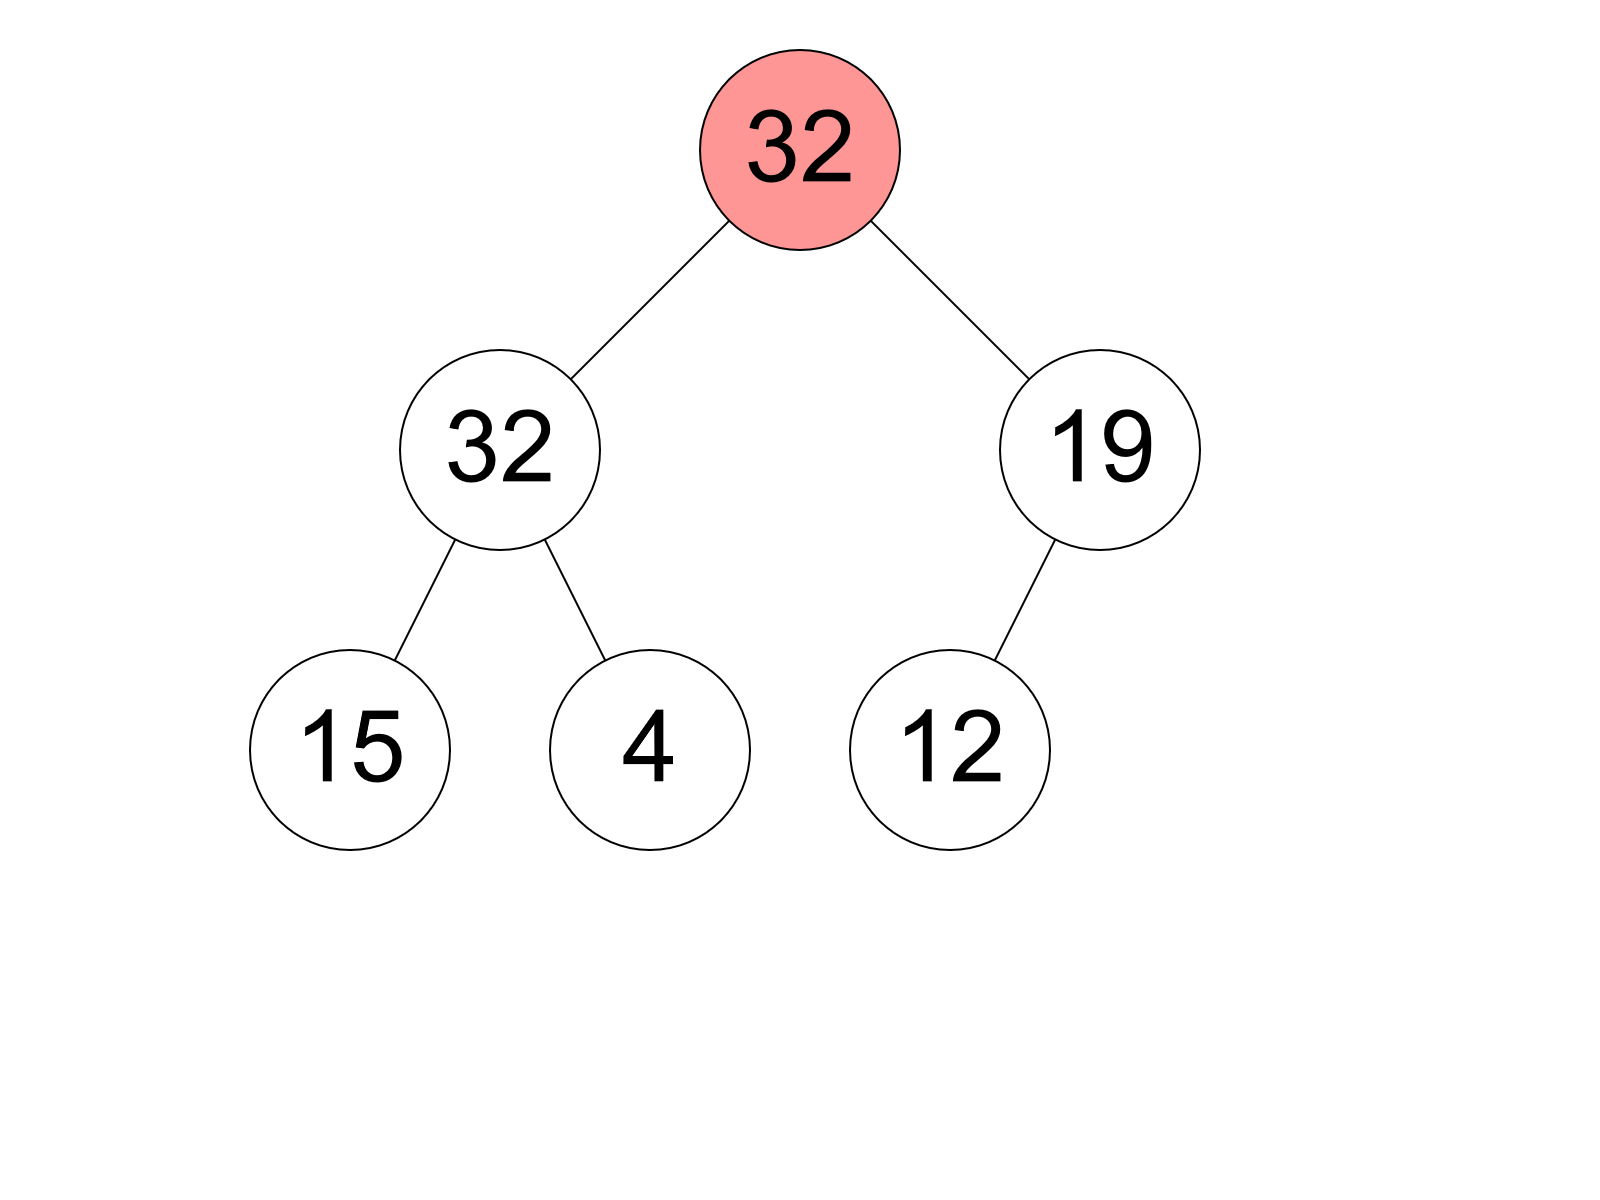
\includegraphics[width=\textwidth]{img/b10}
            \end{subfigure}
            \begin{subfigure}[b]{0.23\textwidth}
                \centering
                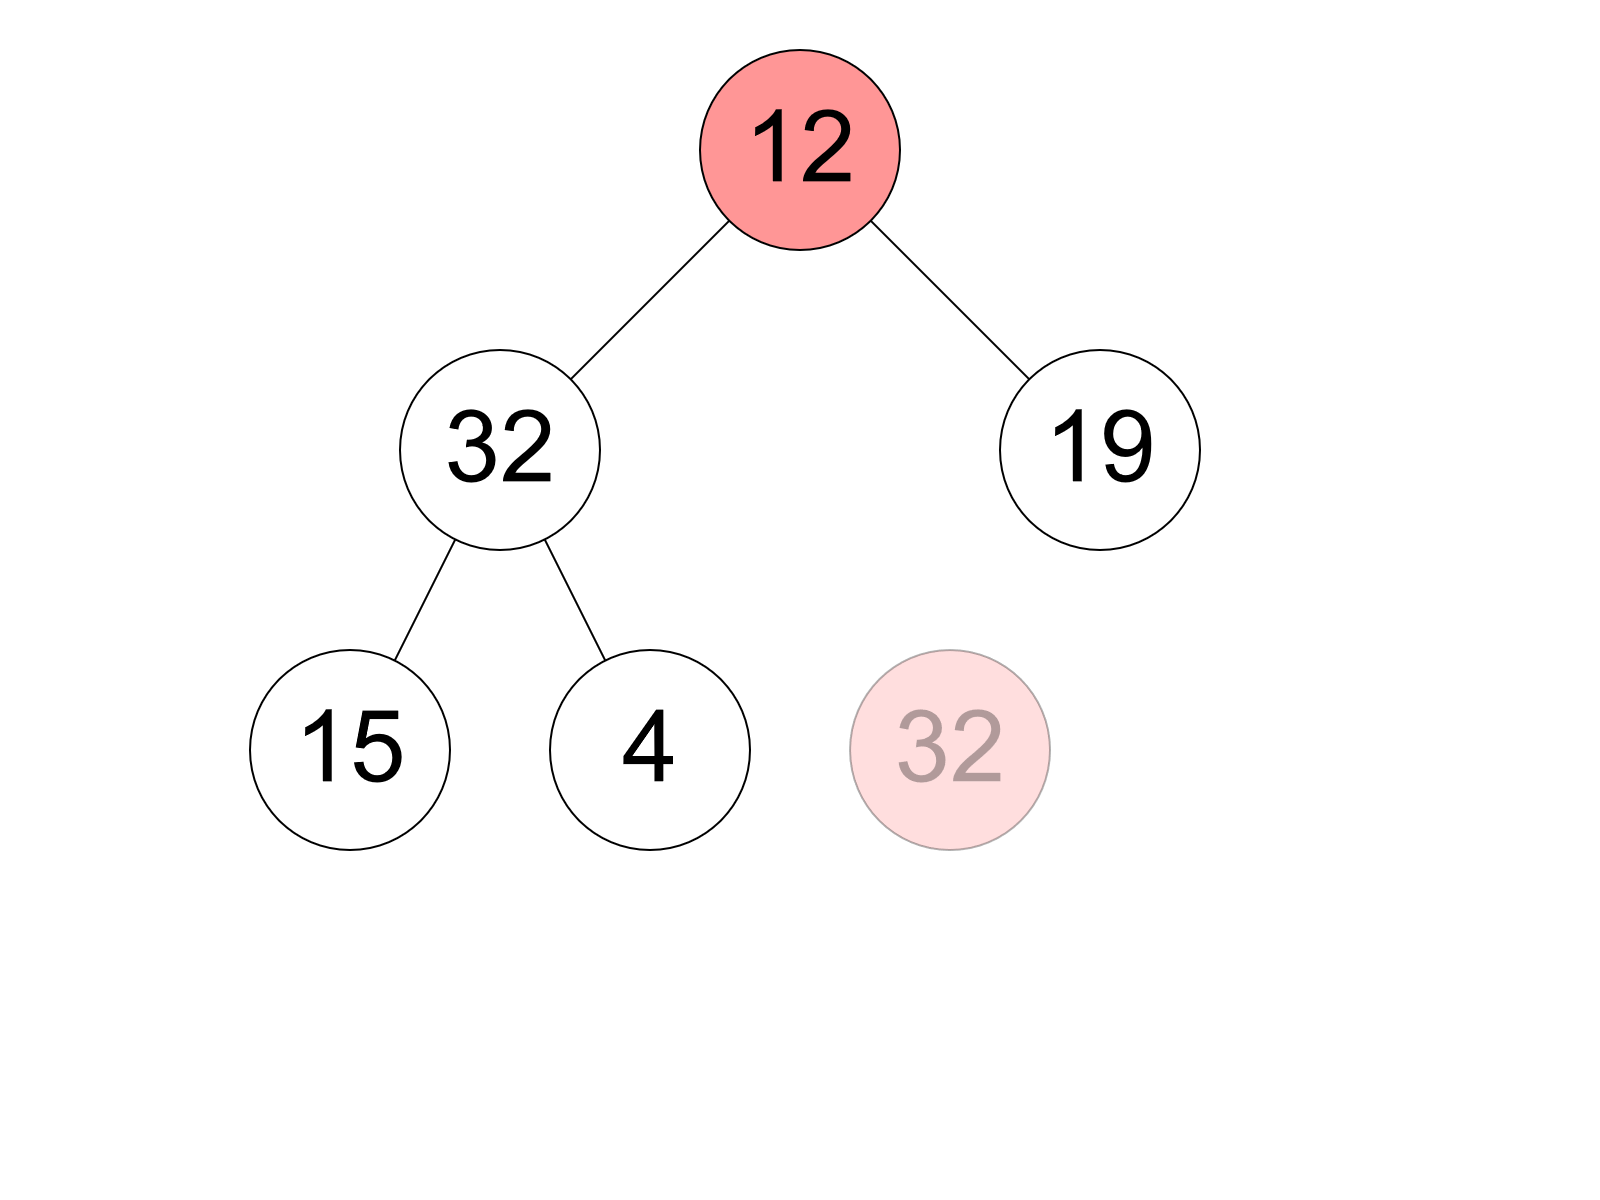
\includegraphics[width=\textwidth]{img/b11}
            \end{subfigure}
            \begin{subfigure}[b]{0.23\textwidth}
                \centering
                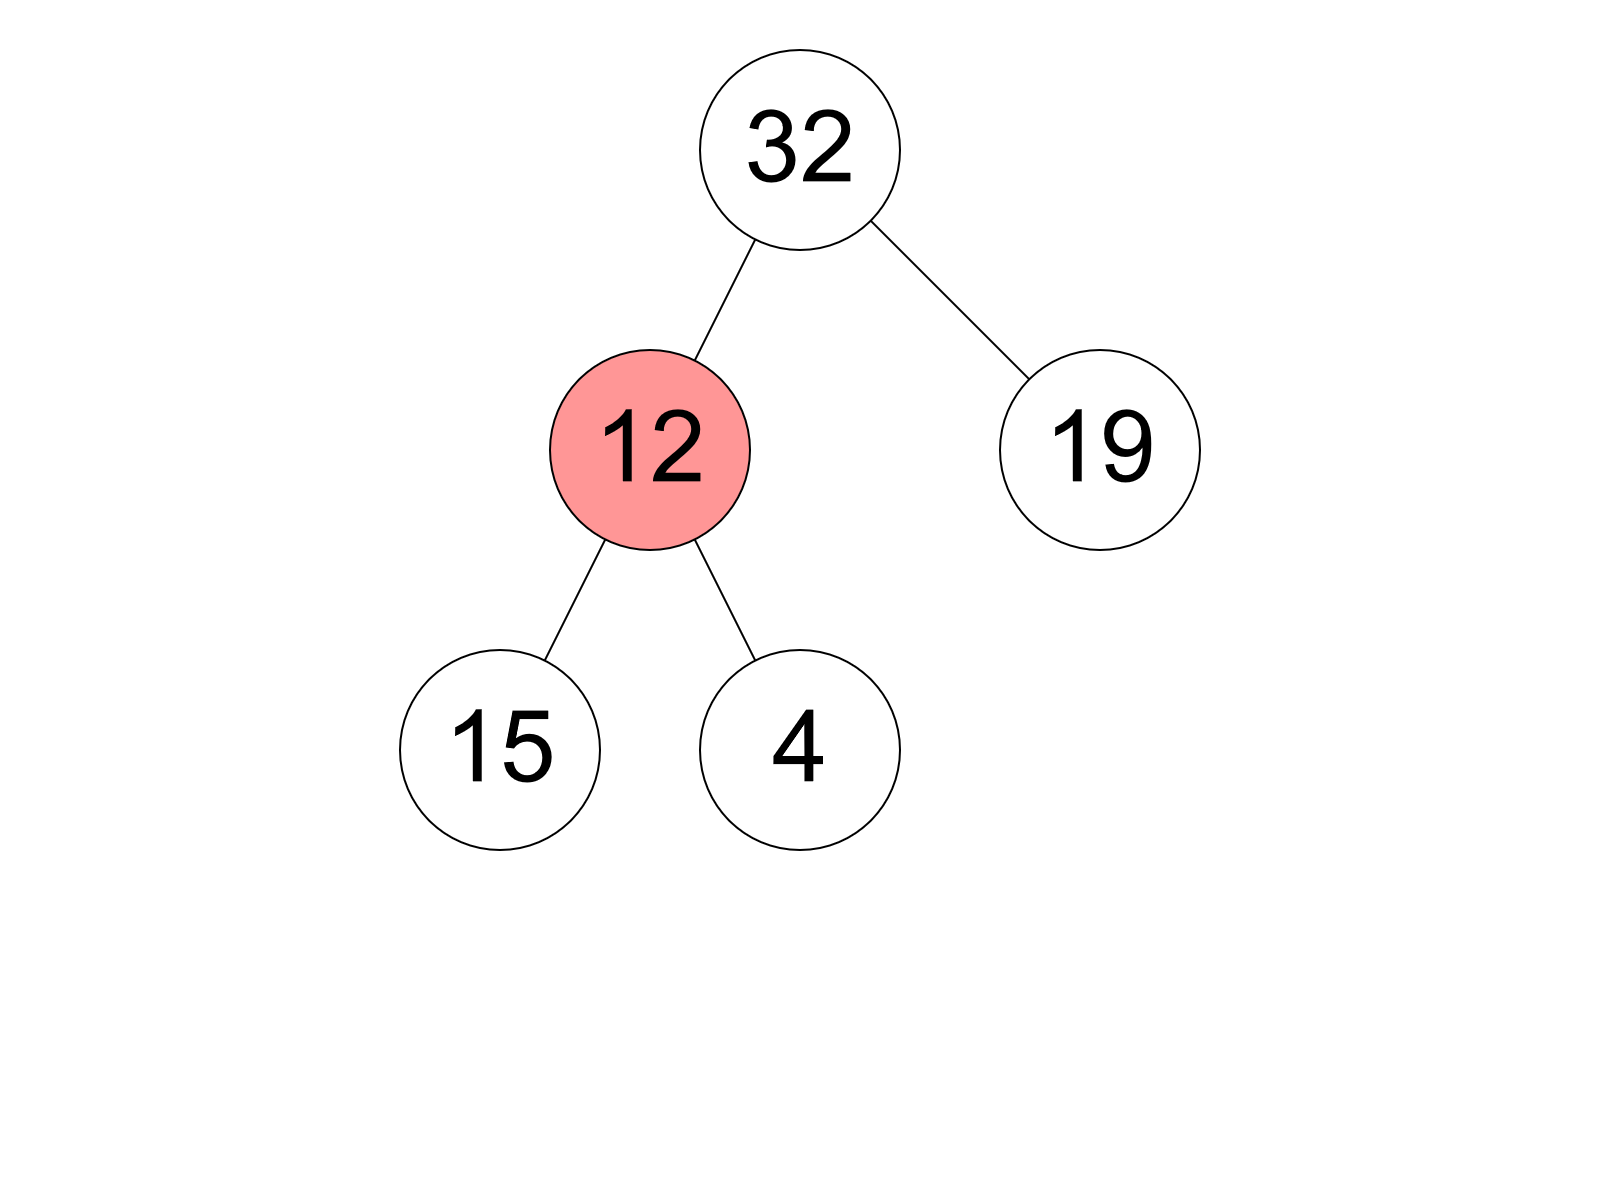
\includegraphics[width=\textwidth]{img/b12}
            \end{subfigure}
            \begin{subfigure}[b]{0.23\textwidth}
                \centering
                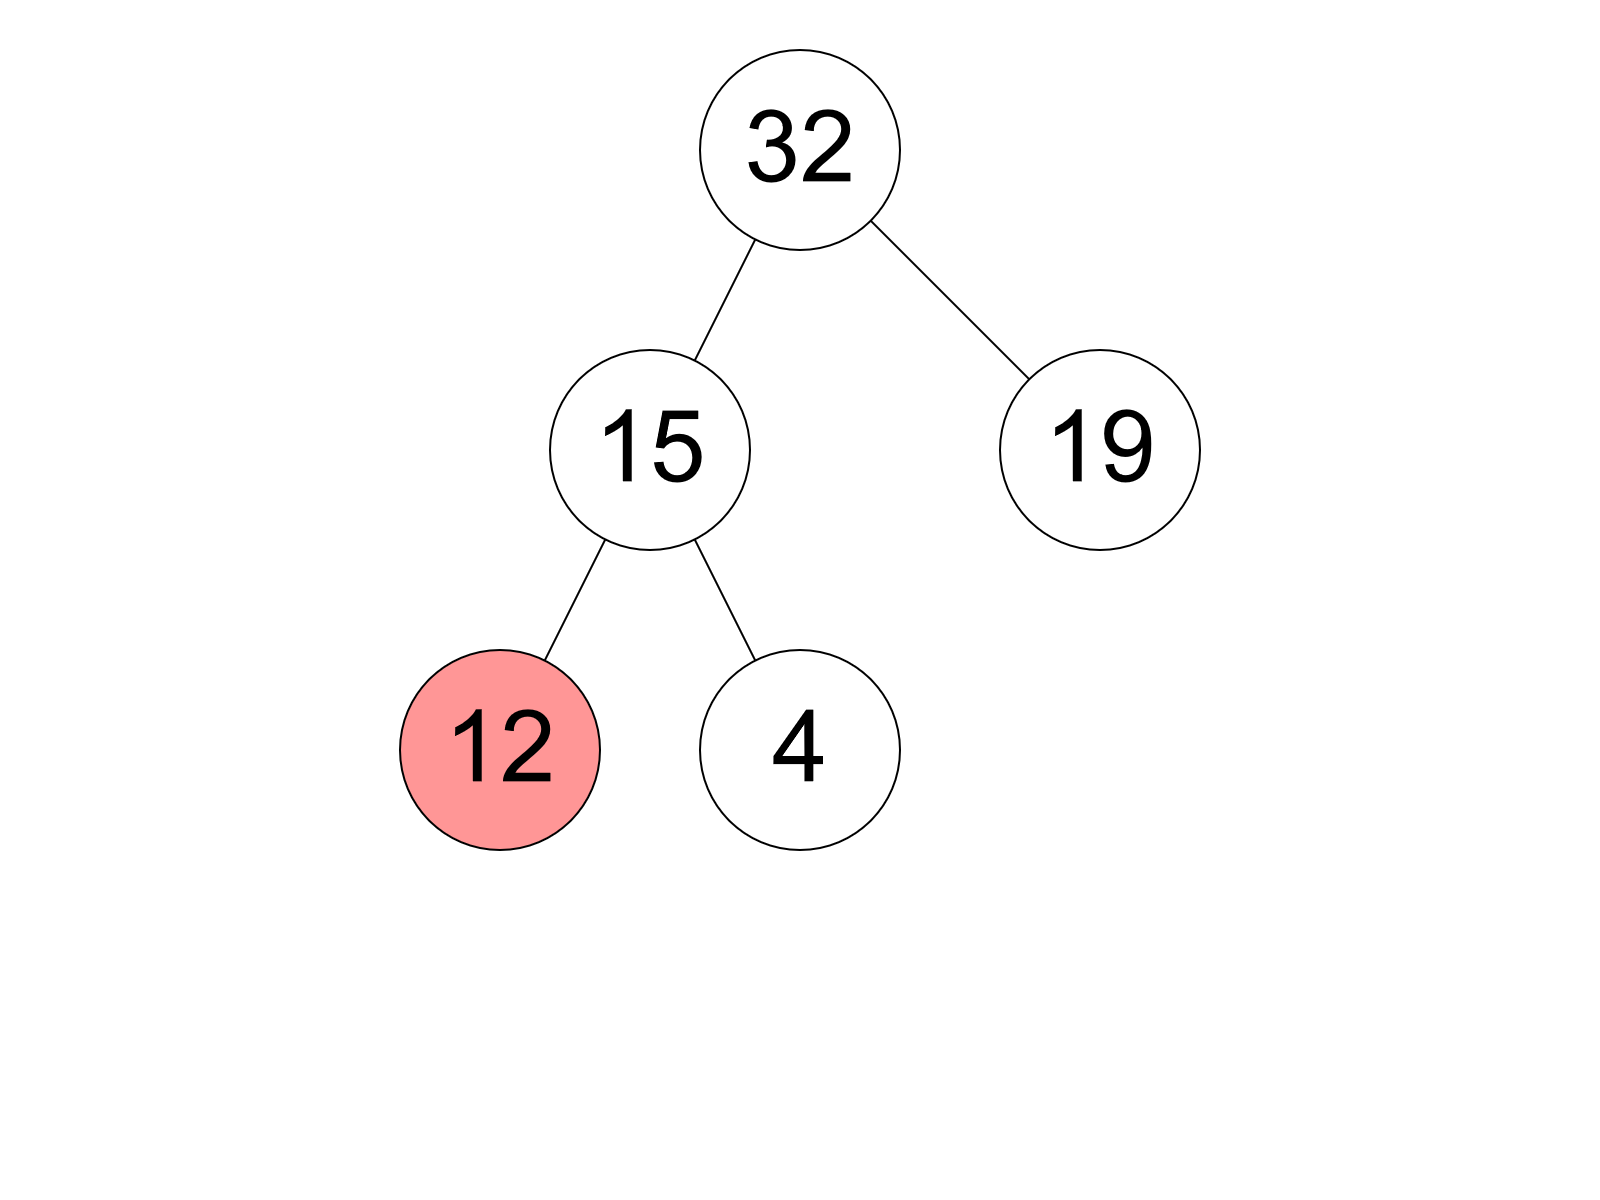
\includegraphics[width=\textwidth]{img/b13}
            \end{subfigure}
        \end{figure}
        \FloatBarrier
        
        \ifcsdef{showLoesung}{\newpage}{}

        \item 
        Die Laufzeit von \textsc{BubbleUp} ist beschränkt durch die Höhe des Heaps und damit im Worst Case $O\big(\log(n)\big)$.
        \begin{description}
            \item[\textsc{Remove}] 
            Um ein Element zu entfernen, wird analog zu \textsc{ExtractMax} der Wert mit dem letzten Element des Heaps getauscht.
            Ist der \glqq{}hochgetauschte\grqq{} Wert größer als sein Vorgänger, muss auf ihm \textsc{BubbleUp} aufgerufen werden, um die Heap-Eigenschaft wiederherzustellen, anderenfalls \textsc{Heapify}.
            \begin{samepage}
            \begin{algorithmic}[1]
                \Procedure{Remove}{$a, l, i$}
                    \State \textsc{Swap}$(n - 1, i)$.
                    \State \textsc{BubbleUp}$(a, i)$.
                    \State \textsc{Heapify}$(a, l - 1, i)$
                \EndProcedure
            \end{algorithmic}
            \end{samepage}
            Sowohl \textsc{BubbleUp} als auch \textsc{Heapify} haben Worst-Case-Laufzeit $O\big(\log(n)\big)$.

            \item[\textsc{Insert}]
            Um ein Element in den Heap einzufügen, wird dieses nach das aktuell letzte Element in den Heap eingefügt.
            Auf diese Weise wird die Linksvollständigkeit nicht verletzt.
            Anschließend wird das eingefügte Element mittels \textsc{BubbleUp} im Heap nach oben \glqq{}gezogen\grqq{}, bis es an der richtigen Position steht. Dadurch wird die Heap-Eigenschaft wiederhergestellt.
            \begin{samepage}
            \begin{algorithmic}[1]
                \Procedure{Remove}{$a, l, v$}
                    \State $a[l + 1] \gets v$
                    \State \textsc{BubbleUp}$(a, l + 1)$.
                \EndProcedure
            \end{algorithmic}
            \end{samepage}
            Die Worst-Case-Laufzeit von \textsc{Insert} ist die gleiche wie die von \textsc{BubbleUp}, nämlich $O\big(\log(n)\big)$.
        \end{description}

        \item \ \\
        \begin{figure}[h!]
            \centering
            \begin{subfigure}[b]{0.23\textwidth}
                \centering
                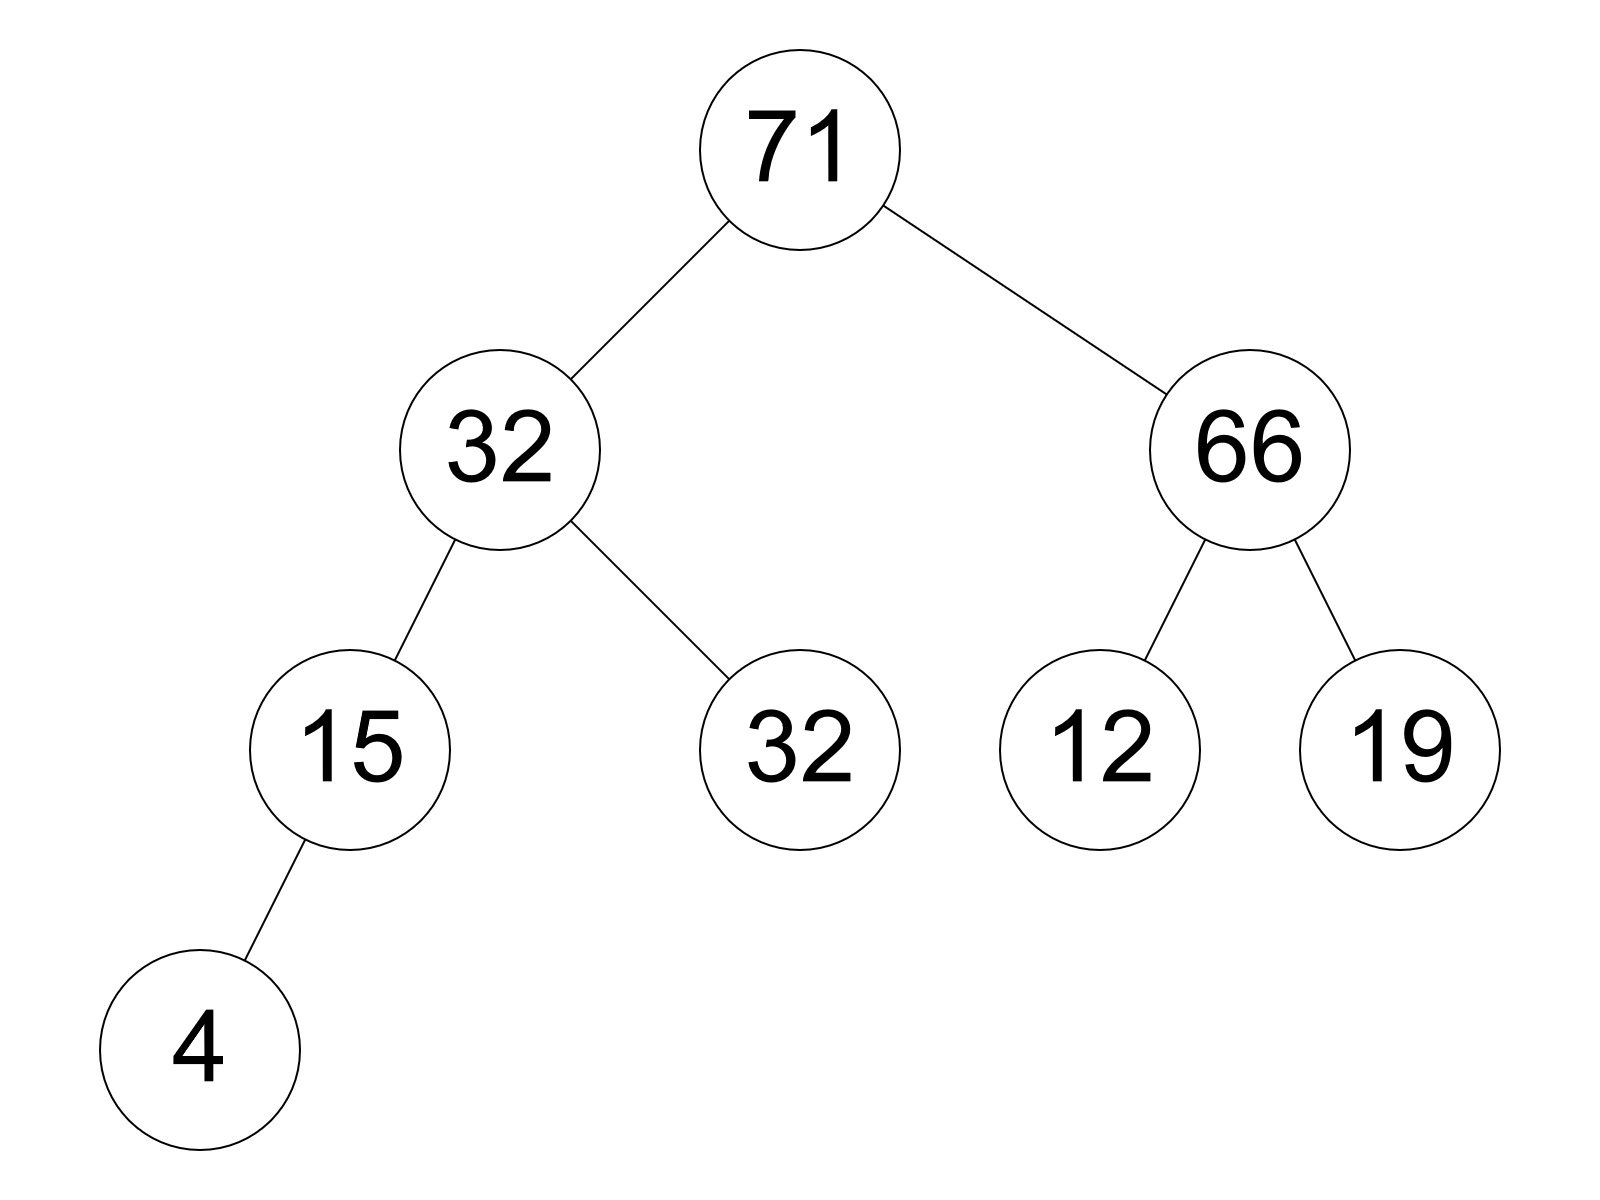
\includegraphics[width=\textwidth]{img/d1}
            \end{subfigure}
            \begin{subfigure}[b]{0.23\textwidth}
                \centering
                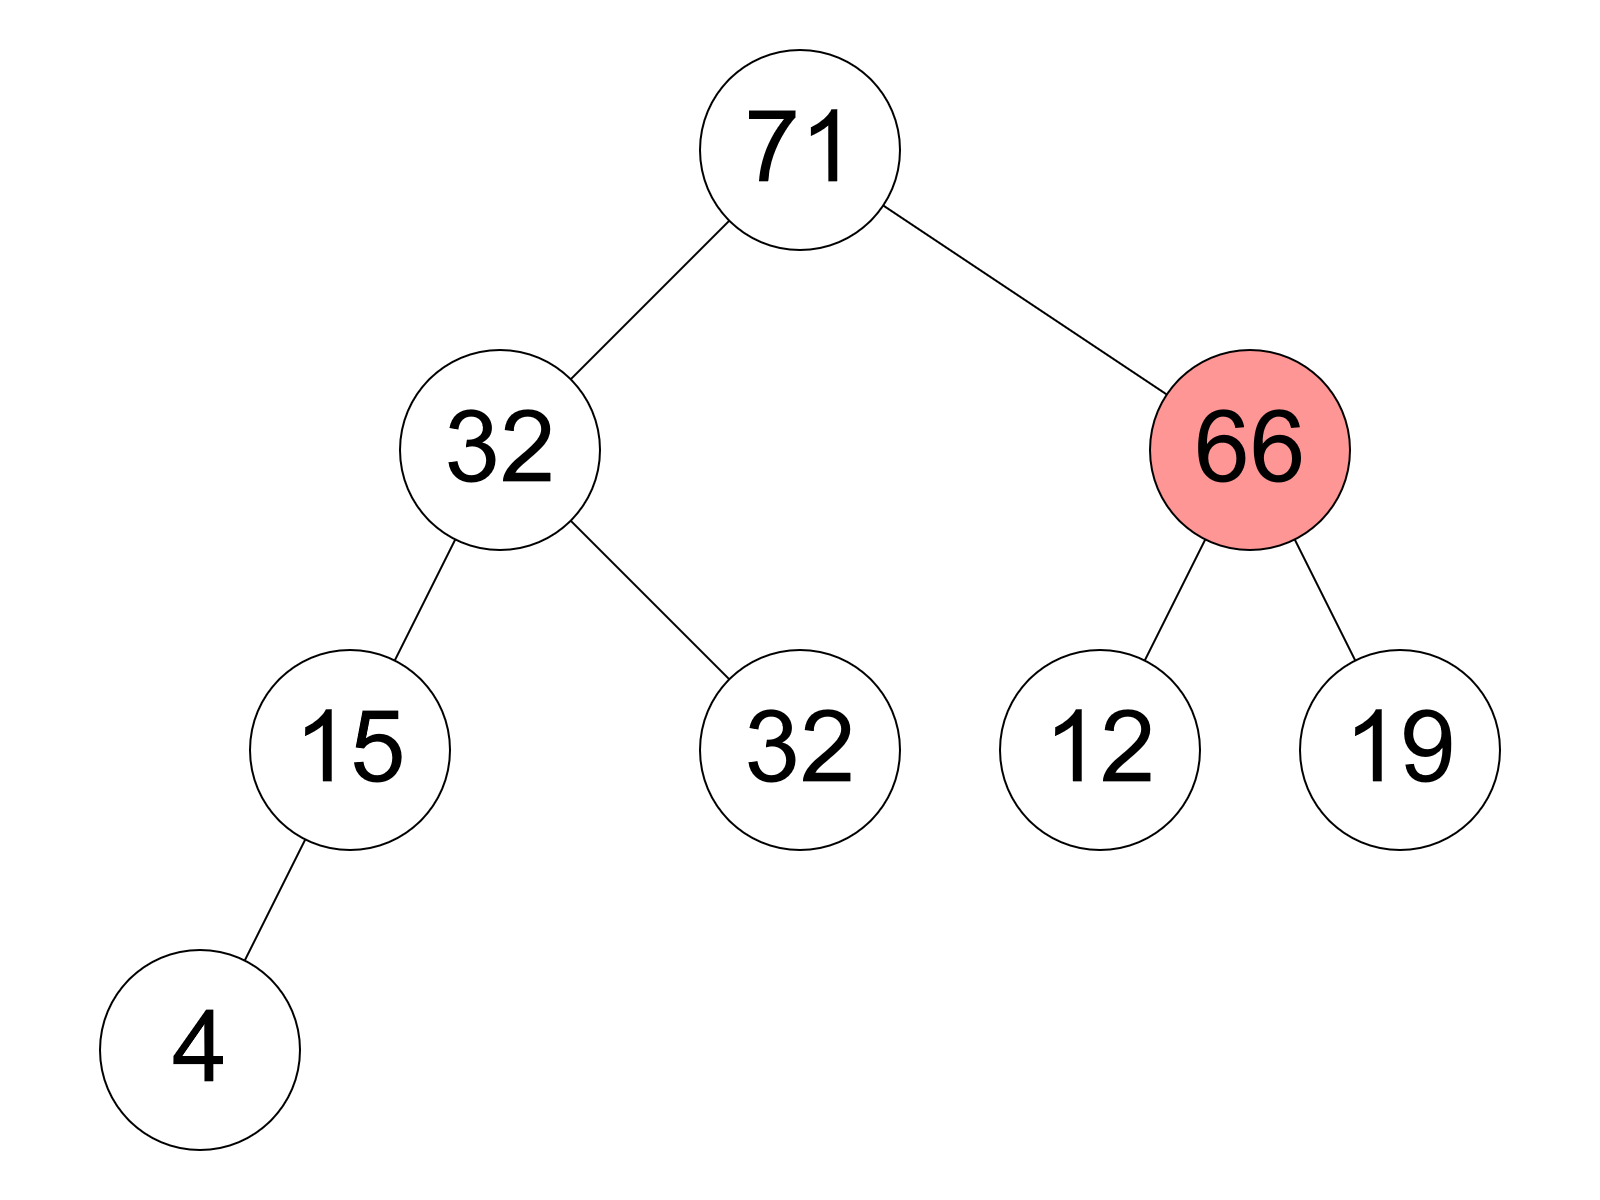
\includegraphics[width=\textwidth]{img/d2}
            \end{subfigure}
            \begin{subfigure}[b]{0.23\textwidth}
                \centering
                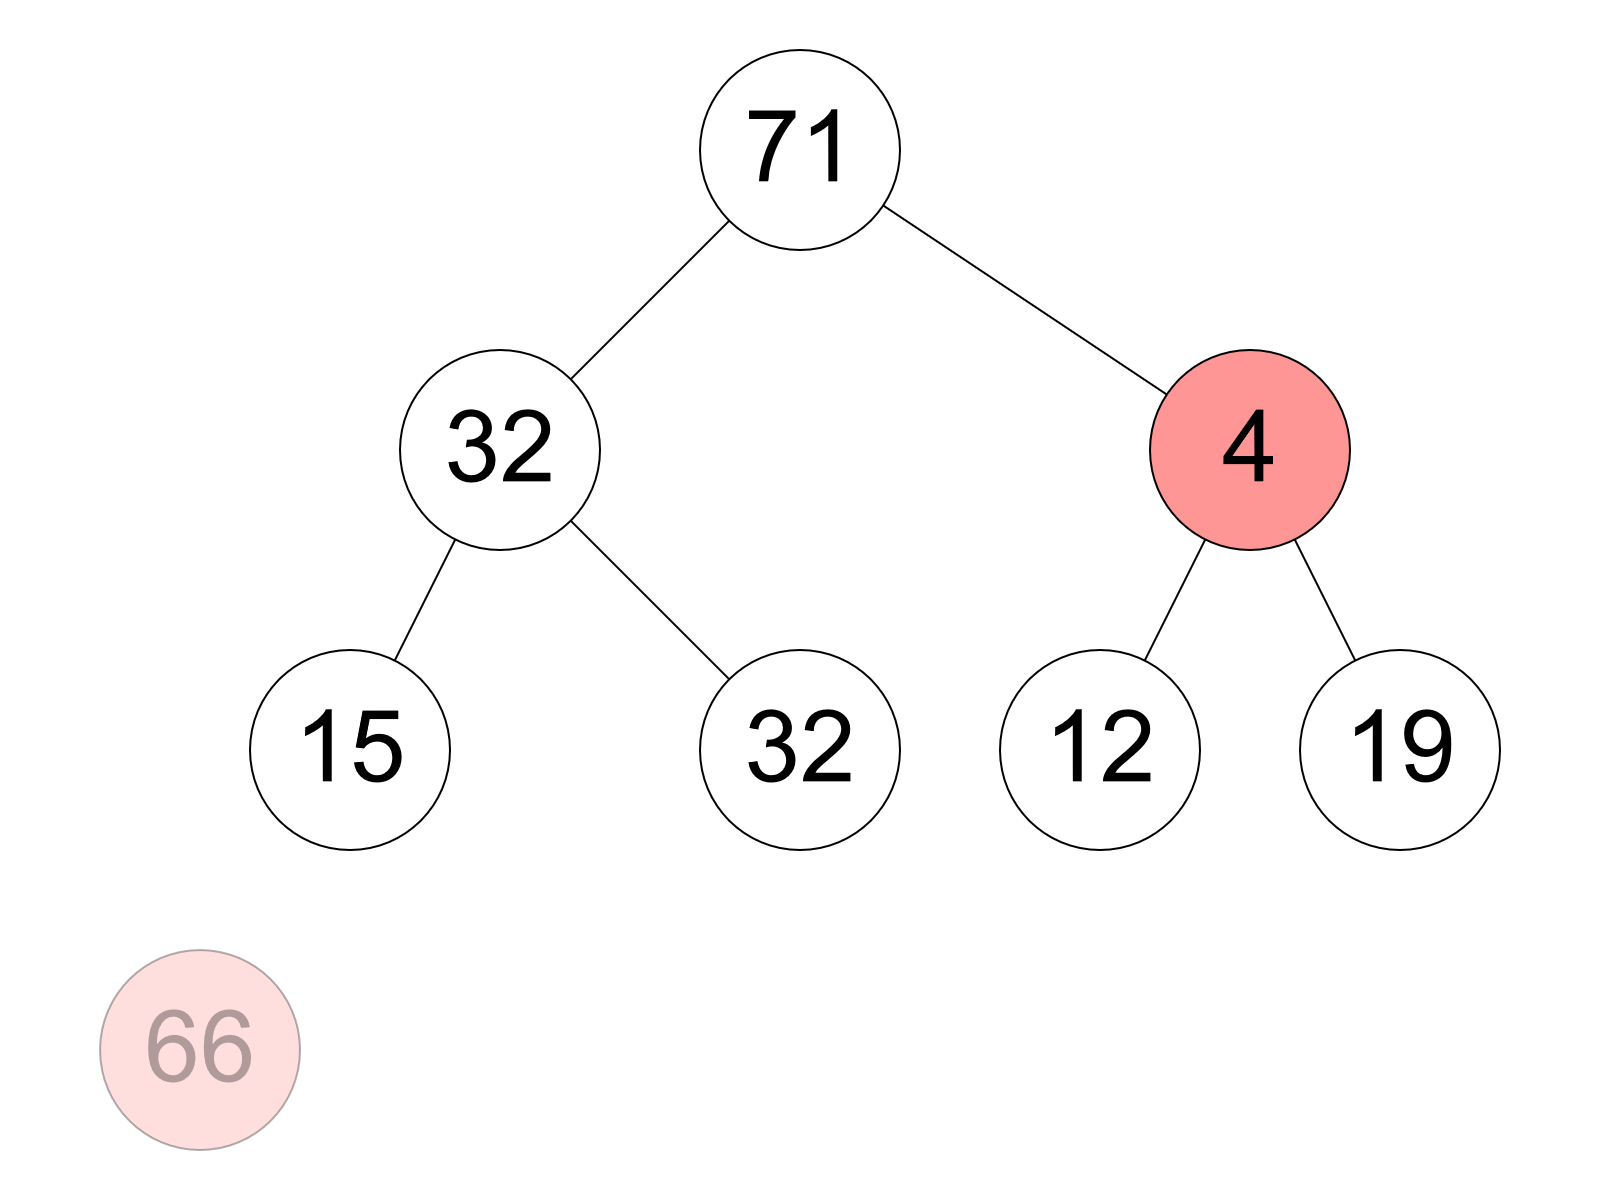
\includegraphics[width=\textwidth]{img/d3}
            \end{subfigure}
            \begin{subfigure}[b]{0.23\textwidth}
                \centering
                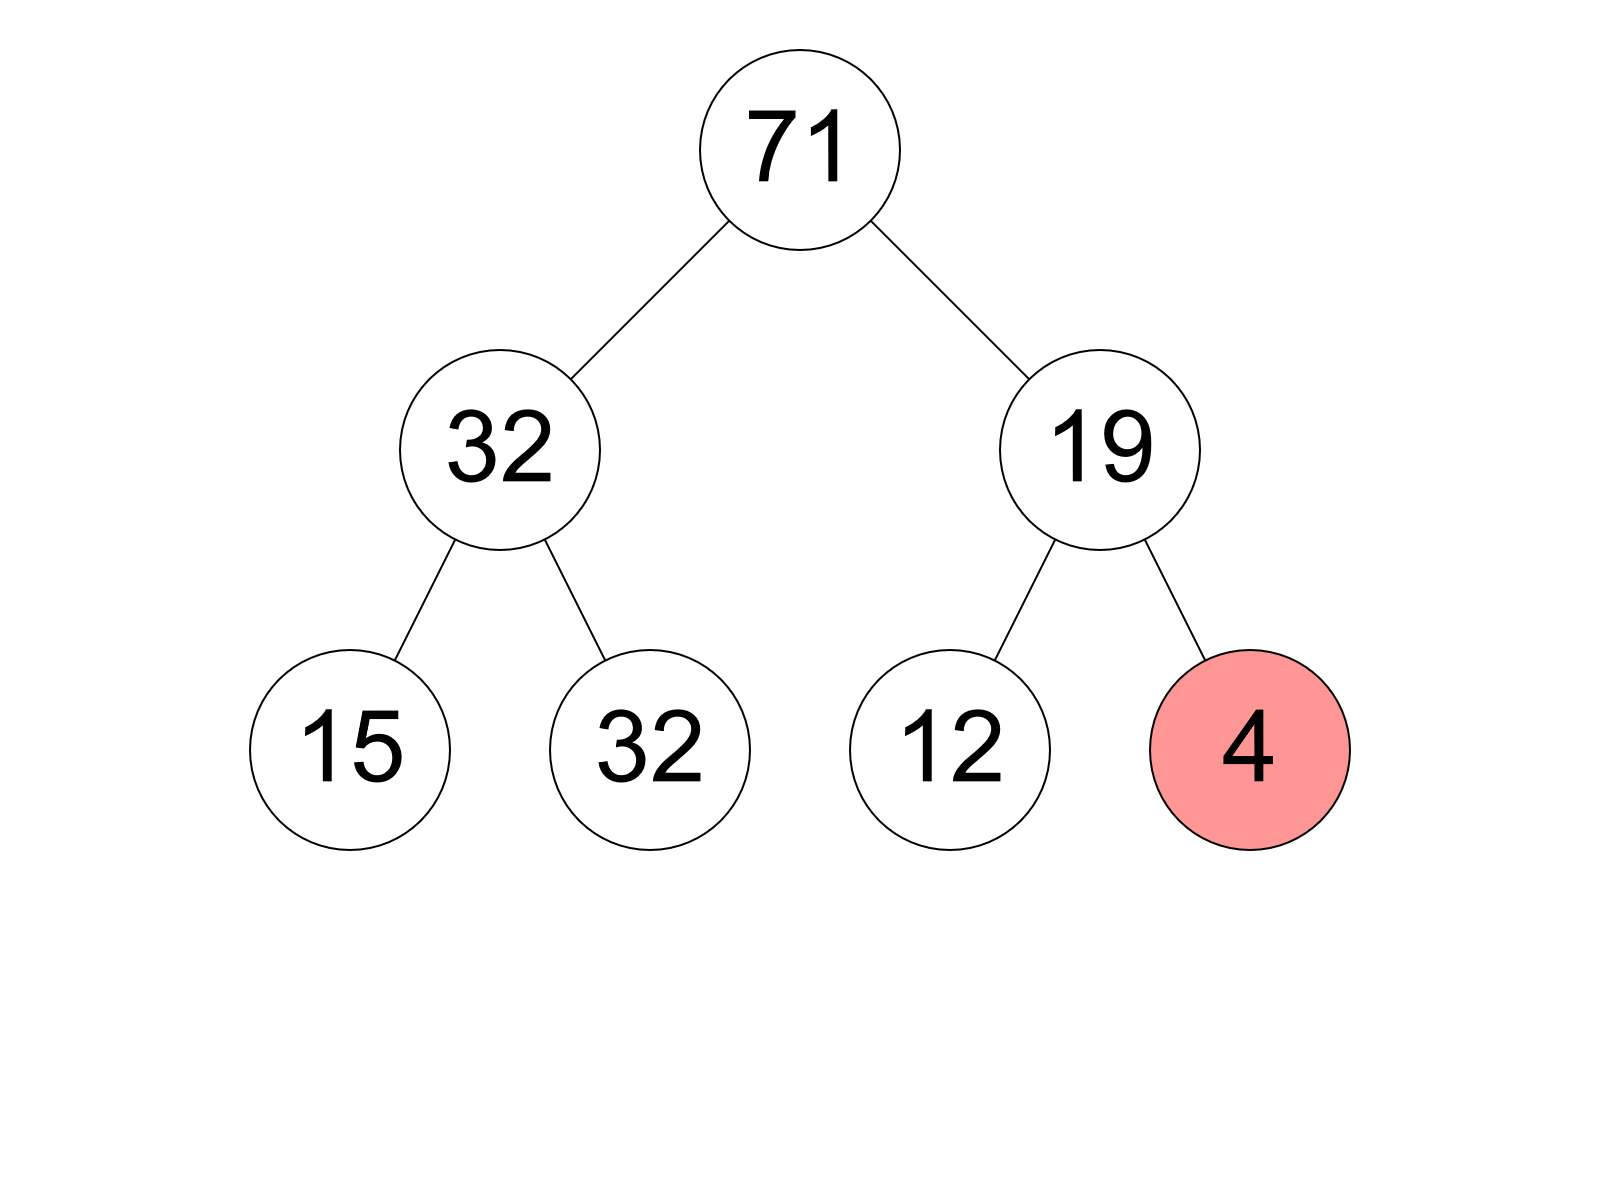
\includegraphics[width=\textwidth]{img/d4}
            \end{subfigure}
            \\
            \begin{subfigure}[b]{0.23\textwidth}
                \centering
                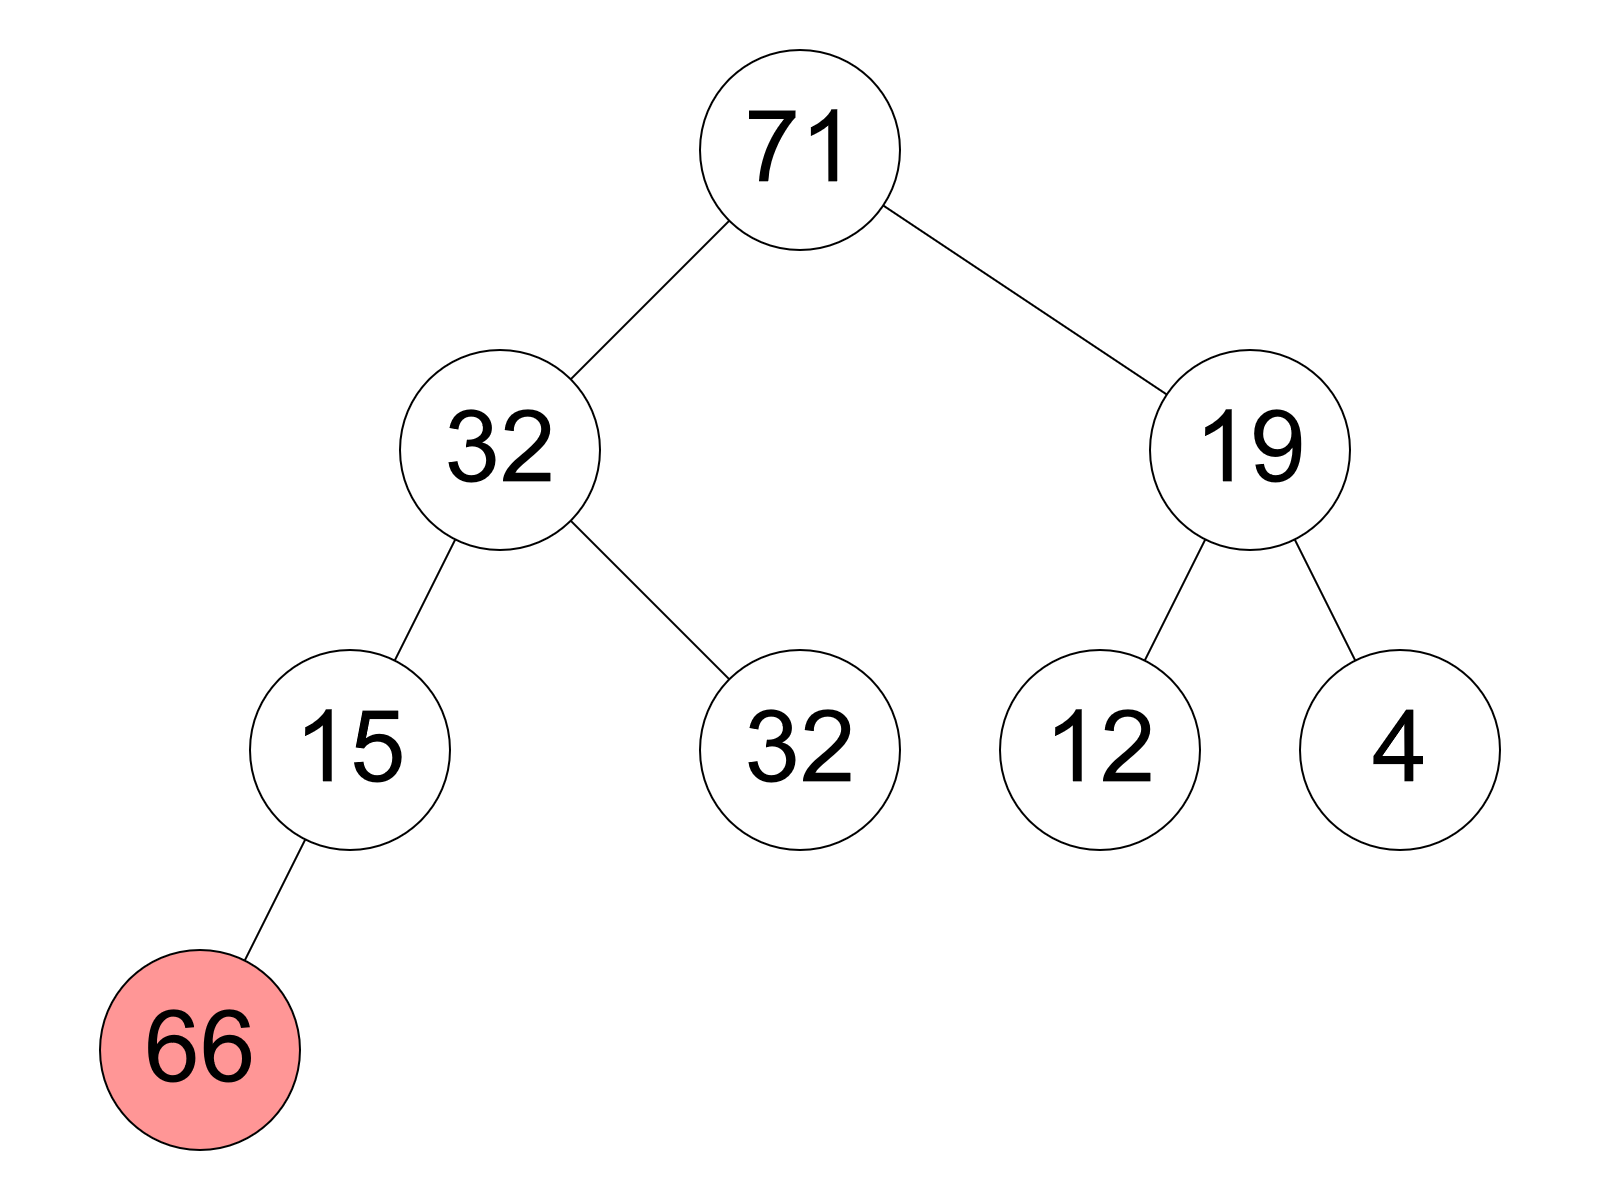
\includegraphics[width=\textwidth]{img/d5}
            \end{subfigure}
            \begin{subfigure}[b]{0.23\textwidth}
                \centering
                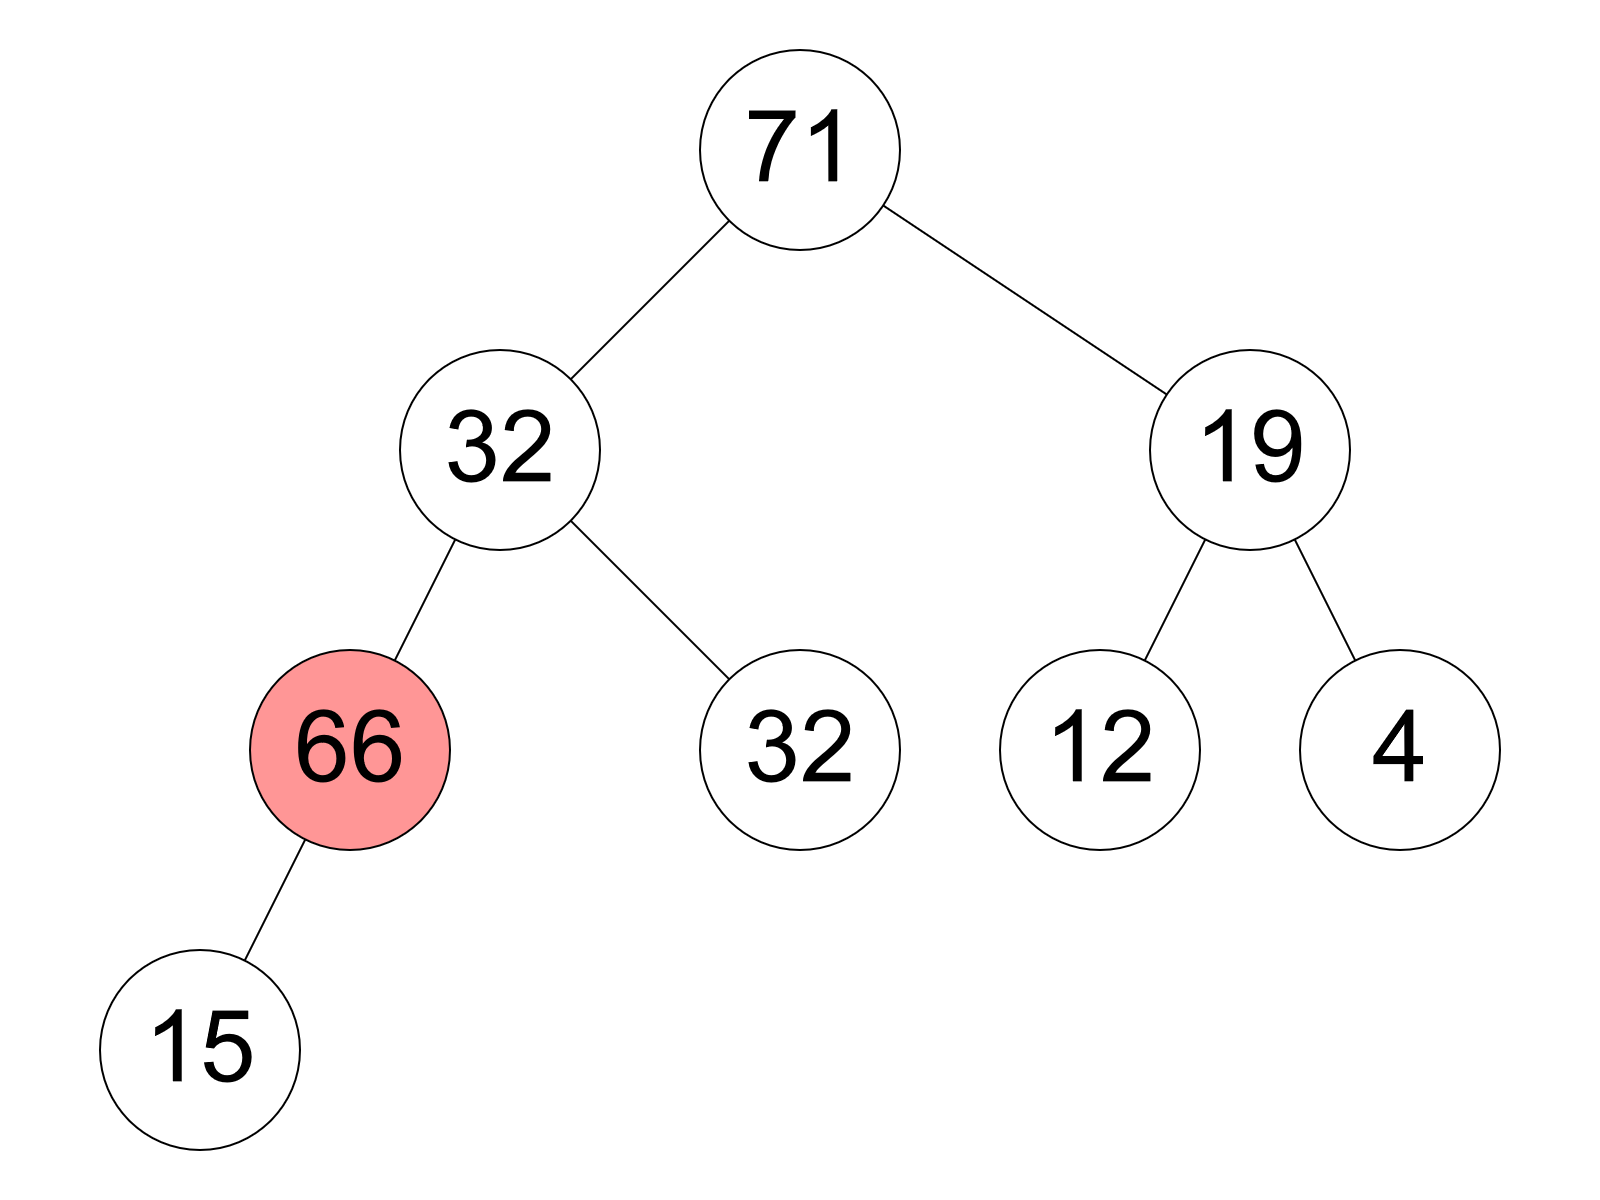
\includegraphics[width=\textwidth]{img/d6}
            \end{subfigure}
            \begin{subfigure}[b]{0.23\textwidth}
                \centering
                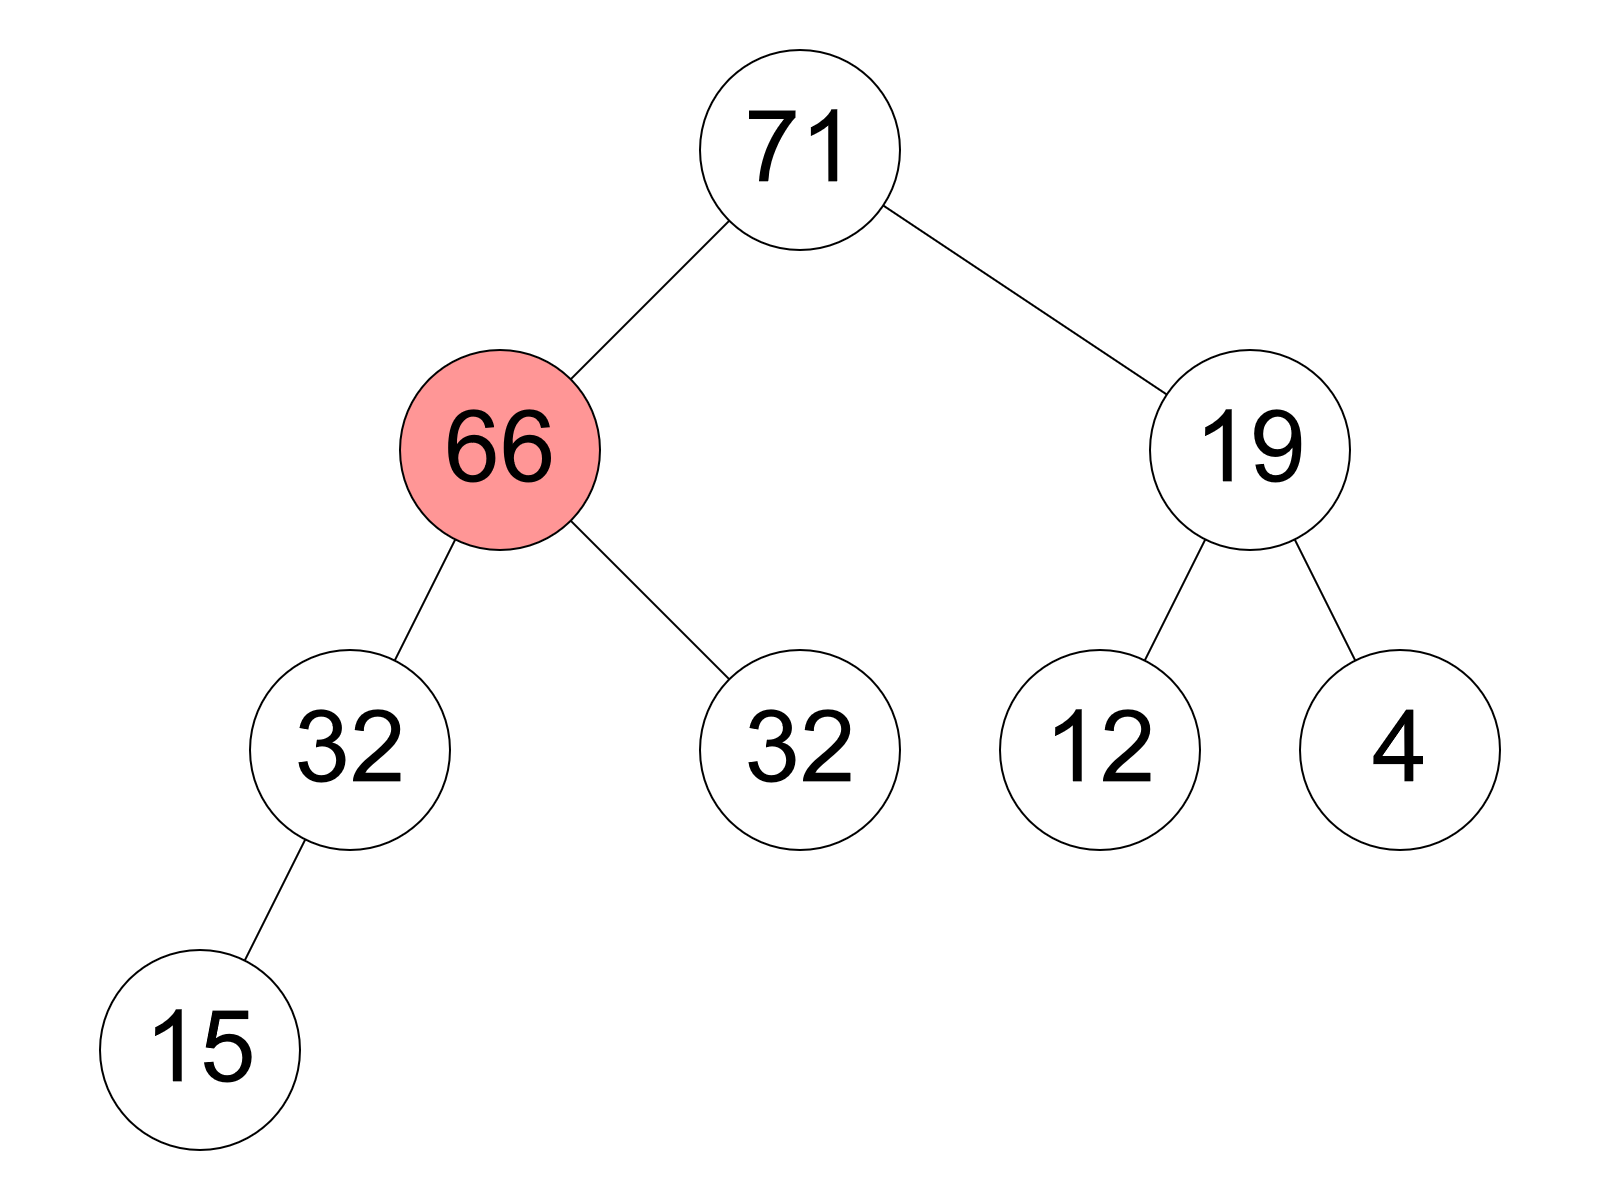
\includegraphics[width=\textwidth]{img/d7}
            \end{subfigure}
        \end{figure}
        \FloatBarrier


    \end{enumerate}
    
\end{loesung}

\begin{aufgabe}{2}{Optimierungen von Mergesort}
    \begin{enumerate}
        \item Sortieren Sie händisch das Array aus Aufgabe 1a) mittels Mergesort.
        Geben Sie den Inhalt des Arrays nach jedem Aufruf von \texttt{merge} an.
        \item Mergesort hat, anders als zum Beispiel Insertionsort, selbst im Best-Case nur eine Laufzeit von $\Theta\big(n \log(n)\big)$.

        Verändern Sie Ihre Mergesort-Implementierung.
        Prüfen Sie dafür vor jedem Aufruf von \texttt{merge} mit einer passenden Bedingung in konstanter Zeit, ob ein Vereinigen überhaupt notwendig ist.
        Falls kein Merge notwendig ist, da dieser Teil des Arrays bereits sortiert ist, überspringen Sie diesen.

        Wie sieht eine Best- und wie eine Worst-Case-Eingabe für die veränderte Mergesort-Implementierung aus?
        Wie lautet nun die Best- und die Worst-Case-Laufzeit?
        \item Um ein Array mit $2n$ Elementen, welches aus zwei sortierten Teilarrays mit jeweils $n$ Elementen besteht, mit der Merge-Operation aus der Vorlesung zu vereinigen, ist ein zusätzliches Array mit Länge $2n$ nötig.
        Verändern Sie die Merge-Operation, sodass Sie nur noch ein Array der Länge $n$ benötigen. Die Laufzeit von $O(n)$ soll sich dabei nicht ändern.
        \begin{description}
            \item[Tipp:] Kopieren Sie zunächst einen Teil der Eingabe in das temporäre Array und vereinigen Sie dann in das ursprüngliche Array hinein.
        \end{description}
    \end{enumerate}
    
\end{aufgabe}

\begin{loesung}
    \begin{enumerate}
        \item \ \\
        \begin{table}[h!]
            \centering
            \begin{tabular}{|c|}
            \hline
            \textbf{Mergesort} \\ \hline
                $(4, 32, 12, 71, 32, 66, 19, 15)$ \\ \hline
                $(4, 32, 12, 71, 32, 66, 19, 15)$ \\ \hline
                $(4, 12, 32, 71, 32, 66, 19, 15)$ \\ \hline
                $(4, 12, 32, 71, 32, 66, 19, 15)$ \\ \hline
                $(4, 12, 32, 71, 32, 66, 15, 19)$ \\ \hline
                $(4, 12, 32, 71, 15, 19, 32, 66)$ \\ \hline
                $(4, 12, 15, 19, 32, 32, 66, 71)$ \\ \hline
            \end{tabular}
        \end{table}

        \item
        Da vor dem \texttt{merge}-Aufruf sowohl das linke als auch das rechte Array bereits sortiert sind, reicht es zu prüfen, ob der rechteste Wert des linken Teilarrays kleiner als der linkeste des rechten Teilarrays ist. Falls ja, kann der Merge übersprungen werden.
        \begin{lstlisting}[language=c++]
void mergesort(int a[], int f, int l){
    if (f < l) {
        int m = (f + l + 1) / 2;
        mergesort(a, f, m - 1);
        mergesort(a, m, l);
        if (a[m - 1] > a[m])
            merge(a, f, l, m);
    }
} 
        \end{lstlisting}
        Bei dieser Optimierung wäre eine Best-Case-Eingabe ein bereits aufsteigend sortiertes Array.
        Hier würde die Bedingung in Zeile 6 stets \emph{wahr} liefern.
        Da in diesem Fall gar kein Vereinigen nötig ist, kann die Laufzeit durch die Rekursionsgleichung $T(n) = 2 T(n / 2) + 1$ angegeben werden.
        Die Master-Methode ($a = 2$, $b = 2$, $f(n) = 1$ $\Rightarrow$ Fall 1) liefert als Laufzeit $\Theta(n)$.

        Eine Worst-Case-Eingabe wäre etwa bei einem absteigend sortierten Array gegeben, bei der zusätzlich alle Werte verschieden sind (bei z.B. nur gleichen Werten ist das Array sowohl ab- als auch aufsteigend sortiert).
        Hier liefert die Bedingung in Zeile 6 immer \emph{falsch}.
        Die Laufzeit ändert sich in diesem Fall nicht wesentlich im Vergleich zur Ursprungsimplementierung, da zusätzlich zur linearen Laufzeit des Vereinigens nur eine weitere Bedingung pro rekursiven Aufruf hinzukommt.
        Die Laufzeit ist also, wie beim ursprünglichen Mergesort, durch $T(n) = 2 T(n / 2) + \Theta(n)$ gegeben.
        Sie bleibt also bei $\Theta\big(n \log(n)\big)$, was sich etwa leicht durch die Mastermethode (Fall 2) zeigen lässt.

        \item 
        Das linke Teilarray wird in das temporäre Array kopiert. Anschließend wird wie gehabt vereinigt.
        Dafür wird für das linke Teilarray aus dem temporären Array gelesen und für das rechte aus dem Ursprungsarray.
        Geschrieben wird in das Ursprungsarray.

        Dies führt scheinbar zu Problemen, da im Ursprungsarray gleichzeitig gelesen und geschrieben wird und somit Werte im rechten Teilarray überschrieben werden.
        Dies stellt jedoch tatsächlich kein Problem dar.
        Angenommen, der $i$-te Wert wird überschrieben.
        Dann gibt es zwei Möglichkeiten: 
        Entweder der $i$-te Wert wurde bereits in die sortierte Liste eingefügt.
        Dann kann dieser Wert problemlos überschrieben werden.
        Oder der Wert wurde noch nicht eingefügt.
        Wenn der $i$-Wert überschrieben wird, bedeutet das, dass gerade der $i$-te Wert in das sortierte Array eingefügt wird.
        Da jedoch Werte in den beiden Teilarrays immer von links nach rechts eingefügt werden, ist dies, wenn der $i$-te Wert noch nicht eingefügt wurde, nur möglich, wenn vorher die $i - 1$ Werte links des $i$-ten Werts eingefügt wurden.
        Das bedeutet, der $i$-te Wert wird mit sich selbst überschrieben, wodurch selbstverständlich ebenfalls kein Problem entsteht.
        \begin{lstlisting}[language=c++]
void merge(int a[], int f, int l, int m) {
    int i, n = l - f + 1;
    int n1 = m - f;
    int *anew = new int[n1];
    for (i = 0; i < n1; i++)
        anew[i] = a[f + i];
    int a1f = 0, a1l = n1 - 1;
    int a2f = m, a2l = l;
    for (i = f; i <= l; i++) {
        if (a1f <= a1l) {
            if (a2f <= a2l) {
                if (anew[a1f] <= a[a2f])
                    a[i] = anew[a1f++];
                else a[i] = a[a2f++];
            } else a[i] = anew[a1f++];
        } else a[i] = a[a2f++];
    }
    delete [] anew;
}
        \end{lstlisting}

    \end{enumerate}
\end{loesung}

\begin{aufgabe}{3}{Finden der $k$ größten Elemente in einem Array}
    Gegeben sei ein Array mit $n$ paarweise verschiedenen Elementen. Es sollen die $k$ größten Werte in diesem Array in absteigend sortierter Reihenfolge ausgegeben werden.

    \textit{Beispiel:} Bei dem Array $(67, 94, 3, 95, 49, 72, 24, 54, 65)$ und $k = 3$ sollte die Ausgabe $(95, 94, 72)$ lauten.

    Entwickeln Sie drei Algorithmen für dieses Problem, indem Sie jeweils die folgenden Hilfsmittel verwenden:
    \begin{enumerate}
        \item Mergesort
        \item Ein Max-Heap mit den Operationen \textsc{BuildMaxHeap} und \textsc{ExtractMax} (Entfernt mittels \textsc{Heapify} den größten Wert aus dem Heap)
        \item Mergesort, \texttt{preparePartition} sowie der Algorithmus \textsc{QuickSelectLinear}, welcher Ihnen in Worst-Case-Laufzeit $\Theta(n)$ das $k$-größte Element in einem Array von $n$ Werten liefert (siehe dazu auch Aufgabe 5 von Tutoriumsblatt 3).
    \end{enumerate}

    Beschreiben Sie Ihre drei Algorithmen in Pseudocode. Geben Sie außerdem jeweils die Worst-Case-Laufzeit in $O$-Notation abhängig von $n$ und $k$ an.
    Wählen Sie dabei die obere Schranke so, dass sie so nah wie möglich an der tatsächlichen Laufzeit liegt.

    Angenommen $k = 10$. Wie lauten dann die Worst-Case-Laufzeiten der Algorithmen abhängig von $n$?

    Angenommen $k = n / 2$. Wie lauten dann die Worst-Case-Laufzeiten der Algorithmen abhängig von $n$?
\end{aufgabe}

\begin{loesung}
    \begin{enumerate}
        \item Sortiere das Array mittels Mergesort und gib die $k$ größten Elemente aus:
        \begin{algorithmic}[1]
            \Procedure{LargestKElements}{$a, n, k$}
                \State \textsc{MergeSort}$(a, 0, n - 1)$
                \For{$i \gets n - k, n - 1$}
                    \State \textsc{Print}$(a[i])$
                \EndFor
            \EndProcedure
        \end{algorithmic}
        Mergesort hat Laufzeit $\Theta\big(n \log(n)\big)$.
        Die Laufzeit von \textsc{LargestKElements} beträgt dementsprechend $\Theta\big(n \log(n) + k\big)$.
        % Da $k \leq n$, kann man die Laufzeit durch $O\big(n \log(n) + n\big)$ beschränken, was $O\big(n \log(n)\big)$ entspricht.
        Da $1 \leq k \leq n$, kann man die Laufzeit durch $\Omega\big(n \log(n) + 1\big)$ und $O\big(n \log(n) + n\big)$ beschränken.
        In beiden Fällen überwiegt $n \log(n)$.
        Also ist die Laufzeit $O\big(n \log(n)\big)$, unabhängig von $k$.

        \item Erstelle mittels \textsc{BuildMaxHeap} einen MaxHeap aus den Elementen und entferne die $k$ größten Elemente mittels \textsc{ExtractMax}:
        \begin{algorithmic}[1]
            \Procedure{LargestKElements}{$a, n, k$}
                \State \textsc{BuildMaxHeap}$(a, n)$
                \For{$i \gets 1, k$}
                    \State $v \gets \text{\textsc{ExtractMax}$(a, n)$}$
                    \State \textsc{Print}$(v)$
                    \State $n \gets n - 1$
                \EndFor
            \EndProcedure
        \end{algorithmic}
        Die Laufzeit ergibt sich durch \textsc{BuildMaxHeap} ($O(n)$) sowie $k$ Aufrufen von \textsc{ExtractMax} (jeweils $O(\log(n))$).
        Die Laufzeit beträgt also $O\big(n + k\log(n))$.
        Für $k = 10$ überwiegt $n$ gegenüber $10 \log(n)$; die Laufzeit ist also in diesem Fall $O(n)$. 
        Im Falle von $k = n / 2$ überwiegt $n / 2 \log(n) = \Omega\big(n \log(n)\big)$ gegenüber $n$; die Laufzeit beträgt daher $O\big(n \log(n)\big)$.

        \item Finde das $k$-größte Element mittels \textsc{QuickSelectLinear}, partitioniere anhand dieses Elements, sortiere die $k$ größten Elemente mittels Mergesort:
        \begin{algorithmic}[1]
            \Procedure{LargestKElements}{$a, n, k$}
                \State $v \gets \text{\textsc{QuickSelectLinear}$(a, n, k)$}$
                \State $i \gets 0$
                \While{$a[i] \neq v$}
                    \State $i \gets i + 1$
                \EndWhile
                \State \textsc{Swap}$(a[i], a[0])$
                \State \textsc{PreparePartition}$(a, 0, n - 1, i)$
                \State \textsc{MergeSort}$(a, i, n - 1)$
                \For{$j \gets i, n - 1$}
                    \State \textsc{Print}$(a[j])$
                \EndFor
            \EndProcedure
        \end{algorithmic}
        \textsc{QuickSelectLinear}, die \textbf{while}-Schleife und \textsc{PreparePartition} benötigen jeweils Laufzeit $O(n)$.
        Merge\-sort wird nur auf den $k$ größen Elementen aufgeführt und benötigt deshalb Laufzeit $O\big(k \log(k)\big)$. 
        Die Laufzeit des gesamten Algorithmus beträgt also $O\big(n + k\log(k)\big)$.
        Für $k = 10$ beträgt die Laufzeit also $O\big(n + 10\log(10)\big)$, was $O(n)$ entspricht.
        Für $k = n / 2$ beträgt die Laufzeit $O\big(n + n / 2 \log(n / 2))$.
        Da $n / 2 \log(n / 2) = n / 2 \log(n) - n / 2$, entspricht dies $O(n \log n)$.
    \end{enumerate}
\end{loesung}

\begin{aufgabe}{4}{Algorithmus zum Finden der Anzahl von Inversionen in einem Array}
    \textit{Hinweis:} Die folgende Aufgabe baut auf Aufgabe 4 von Tutoriumsblatt 3 auf.
    Es ist hilfreich, diese Aufgabe vorher zu bearbeiten.

    Gegeben sei ein Array $(a_1, a_2, a_3, \ldots a_{n - 1}, a_n)$ mit $n$ Elementen.
    Dann ist eine Inversion definiert als ein Paar $(a_i, a_j)$ von zwei verschiedenen Elementen des Arrays, die in absteigender Reihenfolge im Array liegen.
    Die Menge aller Inversionen eines Arrays ist also gegeben durch $I = \{(a_i, a_j) \mid 1 \leq i < j \leq n \wedge a_i > a_j \}$.

    Entwickeln Sie einen Algorithmus, der in $\Theta(n \log n)$ die Anzahl der Inversionen in einem Array berechnet.
    \begin{description}
        \item[Tipp:] Modifizieren Sie Mergesort. Zählen Sie Inversionen innerhalb der \texttt{merge}-Operation.
        % \item[Tipp 2:] Wenn Sie ein Array in der Mitte in zwei Hälften teilen, liegen die beiden Werte einer Inversion entweder beide in der linken Hälfte, beide in der rechten Hälfte oder ein Wert in der linken und ein Wert in der rechten Hälfte.
    \end{description}
\end{aufgabe}

\begin{loesung}
    Jeder Rekursionsaufruf soll die Anzahl der Inversionen im entsprechenden Teilarray liefern.
    Beim Vereinigen von zwei Teilarrays kommen neben den Inversionen innerhalb der beiden Teilarrays noch die Inversionen hinzu, bei denen sich ein Element im linken und eines im rechten Teilarray befindet.
    Da sich alle Werte des linken Teilarrays links von allen Werten des rechten Teilarrays befinden, bleiben solche Inversionen erhalten, selbst wenn die beiden Teilarrays vorher (durch Mergesort) sortiert wurden.
    Dass die beiden Teilarrays in aufsteigend sortierter Reihenfolge vorliegen, kann beim Zählen ausgenutzt werden.

    Eine Möglichkeit, Invesionen zwischen den beiden Teilarrays zu zählen, ist, für jeden Wert des rechten Teilarrays die Anzahl der Inversionen mit Elementen des linken Teilarrays zu bestimmen und all diese Werte aufzusummieren.
    Für jeden Wert $r$ im rechten Teilarray ist die Anzahl der Inversionen mit Werten des linken Teilarrays durch die Anzahl der Werte $l$ im linken Teilarray gegeben, für die gilt: $l > r$.
    Diese Anzahl lässt sich während des Vereinigens der beiden Arrays wie folgt bestimmen:

    Angenommen, während des Vereinigens werden zwei Werte $a_i$ und $a_j$ verglichen, wobei sich $a_i$ im linken und $a_j$ im rechten Teilarray befindet ($f \leq i \leq m - 1$ und $m \leq j \leq l$).
    Sei außerdem $a_i > a_j$.
    Da das linke Teilarray aufsteigend sortiert ist, gilt dann für alle $k \in \{i, i + 1, \ldots,  m - 1\}$: $a_i \leq a_k$.
    Damit gilt $a_k \geq a_i > a_j$.
    All diese $a_k$ bilden also mit $a_j$ eine Inversion.
    Andererseits gilt für alle $k \in \{f, f + 1, \ldots, i - 1\}$: $a_k \leq a_j$, da diese Werte ja bereits vor $a_j$ einsortiert wurden und dies genau dann passiert, wenn $a_k \leq a_j$.
    Also bilden im linken Teilarray $a_i$ und alle Werte rechts davon eine Inversion mit $a_j$, während Werte links von $a_i$ keine Inversion mit $a_j$ bilden.
    Die Anzahl der Inversionen mit dem linken Teilarray, bei denen $a_j$ involviert ist, beträgt daher genau $m - i$.

    Wenn, wie oben vorausgesetzt, $a_i > a_j$ gilt, wird $a_j$ einsortiert und danach nie wieder betrachtet.
    Somit wird keine Inversion doppelt gezählt.
    Bleibt zu klären, ob Inversionen übersehen werden können.
    Es gibt neben dem Fall, dass $a_i > a_j$, nur einen weiteren Fall, bei dem ein Wert $a_j$ aus dem rechten Teilarray einsortiert wird, nämlich immer dann, wenn bereits alle Werte des linken Teilarrays einsortiert wurden (\texttt{a1f > a1l}).
    Wenn dies der Fall ist, gilt jedoch für all diese Werte $a_k \in \{a_f, a_{f + 1}, \ldots, a_{m - 1}\}$: $a_k \leq a_j$.
    Somit bildet $a_j$ mit keinem Wert aus dem linken Teilarray eine Inversion.
    Da beim Vereinigen alle Werte des rechten Teilarrays einsortiert werden und dies stets durch einen der beiden oben beschriebenen Fälle geschiet, werden keine Inversionen übersehen.
    Wenn keine Inversionen übersehen werden und keine Inversionen doppelt gezählt werden, entspricht die Summe, die durch das Aufsummieren der Werte $m - i$ für $a_i > a_j$ resultiert, genau der Anzahl der Inversionen zwischen den beiden Teilarrays.

    \begin{lstlisting}
int merge(int a[], int f, int l, int m) {
    int i, n = l - f + 1;
    int a1f = f, a1l = m-1;
    int a2f = m, a2l = l;
    int *anew = new int[n];
    int inversions = 0;
    for (i = 0; i < n; i++) {
        if (a1f <= a1l) {
            if (a2f <= a2l) {
                if (a[a1f] <= a[a2f]) {
                    anew [i] = a[a1f++];
                } else {
                    anew[i] = a[a2f++];
                    inversions += m - a1f;
                }
            } else anew[i] = a[a1f++];
        } else anew[i] = a[a2f++];
    }
    for (i = 0; i < n; i++)
        a[f + i] = anew[i];
    delete [] anew;
    return inversions;
}
int countInversions(int a[],int f,int l){
    if (f < l) {
        int m = (f + l + 1) / 2;
        int inversions = 0;
        inversions += countInversions(a, f, m-1);
        inversions += countInversions(a, m, l);
        inversions += merge(a, f, l, m);
        return inversions;
    } else {
        return 0;
    }
}
    \end{lstlisting}

    Die Laufzeit des Algorithmus unterscheidet sich zu der von Mergesort im Wesentlichen nur um konstanten Aufwand innerhalb der \texttt{for}-Schleife in \texttt{merge}.
    Somit bleibt ist die Laufzeit in $\Theta$-Notation identisch zu der von Mergesort, nämlich $\Theta\big(n \log(n)\big)$.
\end{loesung}



\end{document}